%!TeX spellcheck = en_GB

	% Import Flags, Setting and Commands
%!TeX root = ccc_main.tex
%!TeX spellcheck = en_GB

\newif\ifBeamer				% True for Beamer presentation/False for paper
\newif\ifFullVersion		% full version
\newif\ifComments			% comments visible
\newif\ifTableOfContents	% table of contents
\newif\ifAnonymous			% anonymous
\newif\ifAbstract			% hide the abstract if false

%\Beamertrue				% Keep this false by default
\FullVersiontrue
\Commentstrue				
\TableOfContentstrue		
%\Anonymoustrue				% Not Anonymous
%\Abstracttrue				% No abstracts in books

% !TeX spellcheck = en_GB
% !TeX root = ccc_main.tex

	%document class
\ifBeamer
	% Settings for Beamer
	\documentclass{beamer}
	\usetheme{Darmstadt}
	
	% Hide tables abstract ecc...
	\TableOfContentsfalse
	\Abstractfalse
	\Anonymousfalse
\else
	% Settings for the actual paper
	\ifFullVersion
		\documentclass[11pt]{book}
	\else
		\documentclass{book}
		\pagestyle{plain}
	\fi
\fi

\usepackage[utf8]{inputenc}
\usepackage[T1]{fontenc}

	%math packages
\usepackage{
	amsmath,	amssymb,	amsthm,
	amsfonts,	mathtools}

	%graphic/floats packages
\usepackage{
	tikz, 		float,
	placeins, 	graphicx,
	graphics,	xcolor} 
	
	%text formatting
\usepackage{
	verbatim,
	bm}

	%other
\usepackage{
	breakcites,	enumerate,
	array,		comment}

	
\usepackage[]{hyperref}
%\hypersetup{
%	colorlinks
%	%allcolors=black
%	%urlcolor=black
%}

	%cryptocode
\usepackage[
	lambda,			advantage,
	operators,		sets,
	adversary,		landau,
	probability,	notions,
	logic,			ff,
	mm,				primitives,
	events,			complexity,
	asymptotics,	keys
	]{cryptocode}
	
	% Define metadata commands
\newcommand{\myauthor}[1]{
	\ifAnonymous
		\author{}
	\else
		\author{#1}
	\fi}

\newcommand{\myinstitute}[1]{
	\ifAnonymous
		\institute{}
	\else
		\institute{#1}
	\fi}


%==============================================================================%
% COUNTERS

% set how far in the sub[n]subsection the Table of Contents will go
\ifTableOfContents
	\setcounter{tocdepth}{2}
\fi

% set the level in which section numbering occurs
\setcounter{secnumdepth}{1}



% !TeX spellcheck = en_GB
% !TeX root = ccc_main.tex
% EG - my personal command


%==============================================================================%% LOGIC

\newcommand*{\ra}{\: \Rightarrow \:}			%implication
\newcommand*{\lra}{\: \Leftrightarrow \:}		%iff


%==============================================================================%
% TEXT STYLE

\newcommand{\EG}[1]{
	\ifComments
		\textcolor{blue}{(\textbf{EG: #1})}
	\fi} 										%Emanuele's Comment
\newcommand*{\cd}[1]{ \mathsf{#1} }				%sans serif mode, for code
\newcommand{\fullorshort}[2]{					
	\ifFullVersion%
		#1%
	\else%
		#2%
	\fi%
	}
\newcommand{\fullversion}[1]{\fullorshort{#1}{}}
\newcommand{\shortversion}[1]{\fullorshort{}{#1}}


%==============================================================================%
% ALGEBRA

\newcommand*{\trs}{\top\hspace{-.1em}}					%transpose of a vector, matrix
\newcommand*{\vc}[1]{\mathbf{#1}}						%vectors
\newcommand{\gexp}[2]{\left[{#2}\right]_{#1}}			%group exponentiation
\newcommand*{\Ker}{{\mathrm{Ker}}\,}					%kernell
\renewcommand*{\Im}{{\mathrm{Im}}\,}					%image
\renewcommand*{\ker}{\Ker}								%making \ker and \Ker synonims


%==============================================================================%
% SETS

\newcommand*{\G}{\mathbb{G}}							%Group
\newcommand*{\F}{\mathbb{F}}							%Field
\newcommand*{\N}{\mathbb{N}}							%Natural Number
\newcommand*{\Z}{\mathbb{Z}}							%Integers
\newcommand*{\QR}{\mathbb{Q}\mathbb{R}}					%quadratic residues
\newcommand*{\range}[1]{{[#1]}}							%integer between 0 and n - 1
	\newcommand*{\RSverbose}[3]{\cd{RS}_{{#1}, {#2}, {#3}}}	%Reed Solomon code (specifing the field)
	\newcommand*{\RS}[2]{\cd{RS}_{{#1}, {#2}}}				%Reed Solomon code

	%operators & predicates
\newcommand*{\rto}{\prescript{\$}{}{\to}}				%sample from a set, random return
\newcommand*{\rgets}{\gets^{\$}}						%value returned involving randomness
\renewcommand*{\sample}{\rgets}							%override of Cryptocode sample
\newcommand*{\checkrel}[1]{\stackrel{?}{#1}}
\newcommand*{\checkeq}{\checkrel{=}}
\newcommand*{\checkneq}{\checkrel{\neq}}


%==============================================================================%
% METRICS

\newcommand{\hd}{d}										%hamming distance
\newcommand{\hw}[1]{\left\lVert#1\right\rVert}			%hamming weight


%==============================================================================%
% PROBABILITY

\renewcommand*{\prob}[1]{ \Pr \left[ #1 \right] }		%probability
\renewcommand*{\adv}[1]{\cd{Adv}\left(#1\right)}		%Advantage


%==============================================================================%
% PARAMETERS & KEYS

\renewcommand*{\sk}{\cd{sk}}							%secret key
\renewcommand*{\pk}{\cd{pk}}							%public key
\newcommand*{\msk}{\cd{msk}}							%master secret key
\newcommand*{\mpk}{\cd{mpk}}							%master public key
\newcommand*{\ppm}{\cd{pp}}								%public parameter
\newcommand*{\spm}{\cd{sp}}								%secret parameter
\newcommand*{\secp}{\lambda}							%security parameter


%==============================================================================%
% UNIT OF MEASUREMENT

\newcommand*{\byte}{\mathrm{B}}
\newcommand*{\KB}{\mathrm{KB}}
\newcommand*{\MB}{\mathrm{MB}}
\newcommand*{\GB}{\mathrm{GB}}


%==============================================================================%
% ORACLE, MACHINES, GAMES

% random oracle
\newcommand{\ro}[1][]{\mathcal{H}_{#1}}

% ddh
\newcommand{\ddh}[1][]{\cd{DDH}^{#1}}


%==============================================================================%
% ENVIRONMENTS

% pseudocode array
\newenvironment{pcarray}[1]{
	\begingroup
	\renewcommand{\arraystretch}{2}
	\setlength{\tabcolsep}{9pt}
	\begin{tabular}{#1}
	}{
	\end{tabular}
	\endgroup
	}

% theorems
\newtheorem{theorem}{Theorem}[section]
\newtheorem{proposition}[theorem]{Proposition}
\newtheorem{lemma}[theorem]{Lemma}
\newtheorem{corollary}[theorem]{Corollary}

\newtheorem{claim}{Claim}

% claim proof
\newenvironment{claimproof}[1]{
	\begin{proof}[Proof of Claim #1]
	% Remove the final QED symbol
	\renewcommand{\qedsymbol}{}
	}{
	\end{proof}
	}


%==============================================================================%
% PSEUDOCODE

% for primitives and algorithms
\createprocedurecommand{algorithm}{}{}{mode = text, linenumbering}

% pchstack/pcvstack default argument
\pcsethstackargs{space = 8pt}
\pcsetvstackargs{space = 8pt}


%==============================================================================%
% MISCELLANEOUS

\newcommand*{\emptyentry}{\; \cdot \;}

%==============================================================================%
	%Wrong things that just work [use at your own risk]
\newcommand*{\pcextraspace}{\pcskipln \\[-12px]}		%add inline space in cryptocode pseudocode
\newcommand*{\prextraspace}{\\[-12px]}					%add inline space in cryptocode protocols
\newcommand*{\midtall}{\phantom{\Big|} \!\!}			%forces higher brakets in equations


%!TeX root = ccc_main.tex
%!TeX spellcheck = en_GB

\title{Collection of Cryptographic Constructions}
\author{Emanuele Giunta}
\date{\today}
	



\begin{document}

\maketitle

%% Table of Contents
\ifTableOfContents 
	\tableofcontents
	\newpage
\fi

%% Main Body

%===============================================================================
% PART ?: CRYPTOGRAPHIC PRIMITIVES
\part{Cryptographic Primitives}
\chapter{Computational Assumptions}

\chapter{From One Way Functions}
	\section{Hard-Core Predicates}
	\subsection{Goldreich-Levin Predicate}
Following the previous works of \cite{FOCS:BluMic82, FOCS:Yao82a} which provided hard-core predicate for specific (classes of) OWFs, \cite{STOC:GolLev89} showed how to obtain them from any OWF.
This is done first extending a given OWF $f : \{0,1\}^n \to Y$, mapping $(x, r) \mapsto (f(x), r)$ where $r \in \{0,1\}^n$ and later showing that $x^\trs r$ is an hard-core predicate for this function\footnote{We denote $x^\trs r$ the inner-product in $\F_2^n$. In bit operations $x^\trs r = \bigoplus_{i = 1}^n (x_i \wedge r)$.}.
Their result lies on the idea that inverting "often" the later function means learning "many" projections of $x$.

As a warm-up, if an adversary $\mathcal{A}$ could guess the predicate correctly always, then $n$ invocations of $\mathcal{A}(f(x), r_j)$ for $r_1, \ldots, r_n$ being linearly independent vectors in $\F_2^n$ would suffice to reconstruct $x$.
The challenge lies when the adversary only has inverse polynomial advantage.
This can be amplified through majority vote techniques exploiting three facts:
\begin{enumerate}
	\item Given $f(x)$, a vector $u \in \F_2^n$ and $b_j = x^\trs r_j$ for $r_1, \ldots, r_m$ pair-wise independent, we can get $m$ pair-wise independent guesses on $x^\trs u$ by computing $b'_j = \mathcal{A}(f(x), u + r_j) - b_j$.
	
	\item Given $k$ correct values for $a_j = x^\trs s_j$ for $r_1, \ldots, r_k$ independent vectors, those can be expanded into $2^k - 1$ pair-wise independent values $b_i = x^\trs r_i$ trough subset sums (excluding the empty set).
	
	\item Pair-wise independence (on large sample) is sufficient to use a Chebyshev bound on majority voting.
\end{enumerate}
The proving strategy is then to define $\mathcal{B}(y)$ attempting to invert $f(x) = y$. Initially it guesses\footnote{The actual algorithm brute-force search those values.} $k > \log m$ predicates values $a_j = x^\trs s_j$, for uniformly sampled $s_1, \ldots, s_k$.
Then it expand those to $m \approx 2^k - 1$ values $b_j = x^\trs r_j$ with $r_j$ being pair-wise independent.
Finally, it invokes $\mathcal{A}(f(x), e_i + r_j) - b_j$ to obtain $m$ guesses of the bit $x_i = x^\trs e_i$, where $e_i$ is the vector with all entries equal to zero and the $i$-th equal to $1$.
Taking a majority vote for each bit, it obtain a candidate $x^\ast$ whose correctness can be checked testing $f(x^\ast) = y$.

\begin{lemma}
	Given $X_1, \ldots, X_m$ pairwise-independent random variables with Bernoulli distribution\footnote{I.e. $\prob{X_i = 1} = 1/2 + \varepsilon$ and $\prob{X_i = 0} = 1/2 - \varepsilon$.} $\mathrm{B}(1/2 + \varepsilon)$, then calling $X = X_1 + \ldots + X_n$,
	\[
		\prob{
			X \leq \frac{m}{2}
		}
			\; \leq \;
		\frac{1}{4m \varepsilon^2}.
	\]
\end{lemma}
\begin{proof}
	\label{lemm:GolLev89:majority_voting}
	Calling $p = 1/2 + \varepsilon$, by linearity $\mathbb{E}(X) = mp$ and $\mathrm{Var}(X) = m p(p - 1) \leq m/4$, which can be shown as $\mathbb{E}(X_i X_j) = p^2$ from pair-wise independence (with $i \neq j$).
	Using a Chebyshev bound then
	\[
		\prob{X \leq \frac{m}{2}}
			\; \leq \;
		\prob{\left| X - pm \right| \geq  \varepsilon m }
			\; \leq \;
		\frac{m/4}{\varepsilon^2 m^2}
			\; = \;
		\frac{1}{4 m \varepsilon^2}.
	\]
\end{proof}

\begin{theorem}
	\label{theo:GolLev89}
	Let $f : \{0,1\}^n \to \{0,1\}^\ast$ be a OWF.
	Then $F : \{0,1\}^{2n} \to \{0,1\}^\ast$ such that $F(x,r) = (f(x), r)$ is a OWF and $h : \{0,1\}^{2n} \to \{0,1\}$ such that $h(x,r) = x^\trs r$ is an hard-core predicate for $F$.
\end{theorem}
\begin{proof}
	Having given the informal overview we focus on the proof. The algorithm is described in Figure~\ref{prot:GolLev84}.
	
	\begin{figure}[htb]
	\centering
	\algorithm{$\mathcal{B}(y):$}{
		Sample $s_1, \ldots, s_k \rgets \{0,1\}^n$ with $k = \log m + 1$
			\\
		\textbf{For} $a_1, \ldots, a_k \in \{0,1\}$:
			\\
		\t Compute $b_1, \ldots, b_m$ and $r_1, \ldots, r_m$ via non-empty subset sums
			\\
		\t \textbf{For} $i \in \{1, \ldots, n\}$:
			\\
		\t\t Compute $x^\ast_{i,j} \gets \mathcal{A}(y, e_i + r_j) - b_j$
			\\
		\t\t Set $x^\ast_i$ the majority bit among $x^\ast_{i,1}, \ldots, x^\ast_{i, m}$
			\\
		\t Reconstruct $x^\ast \gets (x^\ast_1, \ldots, x^\ast_n)$
			\\
		\t \textbf{If} $f(x^\ast) = y$: \textbf{Return} $x^\ast$
			\\
		\textbf{Return} $\perp$
	}
	\label{prot:GolLev84}
	\caption{$\mathcal{B}$ using $\mathcal{A}$ for the Goldreich-Levin predicate to invert $f$.}
	\end{figure}
	
	Assume $\mathcal{A}$ guesses the given predicate with inverse-polynomial advantage $\varepsilon$, that is, for a random $x$ and $r$, $\prob{\mathcal{A}(f(x), r) \to x^\trs r} \geq 1/2 + \varepsilon$.
	Calling $G = \{x_0 \in \{0,1\}^n \: : \: \prob{\mathcal{A}(f(x_0), r)} \geq 1/2 + \varepsilon/2\}$, then $\prob{x \in G} \geq \varepsilon/2$.
	
	Next we study the iteration of the outer loop in which $\mathcal{B}$ guesses $a_1, \ldots, a_k$ correctly.
	In this case we have that $x_{i,j}^\ast$ are equally distributed, pair-wise independent as $r_j$ are and, as $b_j = x^\trs r_j$,
	\begin{align*}
		\prob{x_i = x^\ast_{i,j}}
			\; &= \;
		\prob{x^\trs e_i = \mathcal{A}(f(x), e_i + r_j) - b_j}
			\; \\ &= \;
		\prob{x^\trs (e_i + r_j) = \mathcal{A}(f(x), e_i + r_j)}
			\; \geq \;
		\frac{1}{2} + \frac{\varepsilon}{2}.
	\end{align*}
	From Lemma~\ref{lemm:GolLev89:majority_voting} we thus get that
	\[
		\prob{x_i \neq x^\ast_i}
			\; \leq \;
		\frac{1}{4m \varepsilon^2}
			\quad \ra \quad
		\prob{x \neq (x^\ast_1, \ldots, x^\ast_n)}
			\; \leq \;
		\frac{n}{4m \varepsilon^2}
	\]
	which, up to fixing $m = n/(2\varepsilon^2)$ that is polynomially bounded, can be set to be smaller that $1/2$.
	As we conditioned on $x \in G$, which occurs with probability $\varepsilon/2$, we conclude that $\mathcal{A}$ inverts $f$ with probability $\varepsilon/4$, which is impossible.
	
	Note that for very small $\varepsilon$ though $m$ may become super-polynomial.
	This is solved as follows:
	Assume toward contradiction there exists $\mathcal{A}$ such that its advantage $\varepsilon$ is \textit{infinitely often}\footnote{A predicate $p(\secp)$ hold infinitely often if $\forall \secp_0 \left( \exists \mu_0 \left( \secp_0 \leq \mu_0 \wedge  p(\mu_0) \right) \right)$.} larger than $\secp^{-c}$ for a constant $c$.
	Then we can define a non-uniform adversary $\mathcal{C}(1^\secp, y)$ for the OWF which aborts if $\varepsilon(\secp) < \secp^{-c}$ and runs $\mathcal{B}$ otherwise.
	When $\mathcal{B}$ is executed it runs in polynomial time in $\secp$ as $m = n/(2\varepsilon^2) \leq n \cdot \secp^{2c}$ in this case. Moreover $\mathcal{C}$'s advantage is $\varepsilon/4 \geq 1/4 \cdot \secp^{-c}$ infinitely often, which is a contradiction.
\end{proof}

\chapter{Pseudo Random Function and Permutation}
	\section{Pseudo Random Functions}
	%!TeX root = ../../ccc_main.tex
%!TeX spellcheck = en_GB

\subsection{Goldreich-Goldwasser-Micali from PRG}
Although apparently stronger, the existence of PRF is equivalent to that of Pseudo Random Generators (PRG) with \textit{good} stretch. 
PRFs trivially yields PRGs.
\cite{FOCS:GolGolMic84} instead proposed a tree-like construction of PRFs from PRGs with an expansion factor of $2$\footnote{This is actually implied by PRGs with an expansion factor $1 + p(\secp)^{-1}$ for a given polynomial $p$ through standard amplification techniques.}.
More precisely, let $G : \{0,1\}^\secp \to \{0,1\}^{2\secp}$ be a PRG.
The idea is to sample an initial PRG seed $s$, which serves as PRF key, and define a tree from consecutive application of $G$ where the left child are first $\secp$ bits of $G$'s output, while the right child are last $\secp$ bits.
This is illustrated for height $2$ in Figure~\ref{fig:GGM84:tree_based_prf}.
To evaluate the PRF on input a bit string $(b_1, \ldots, b_n)$, the leaf corresponding to the path identified by those bits (where $0$ means \textit{left-child} and $1$ means \textit{right-child}) is returned.

\begin{figure}[htb]
	\centering
	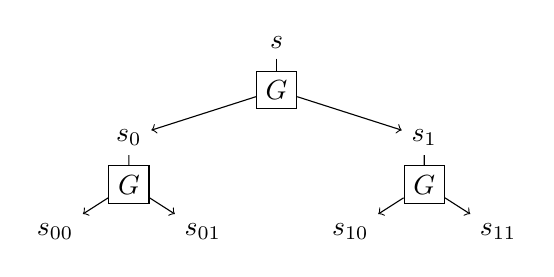
\begin{tikzpicture}[xscale=1.25, yscale=-.6]
		\node (s) at (0,0) {$s$};
		
		\node[draw] (gs) at (0,1) {$G$};
		
		\node (s0) at (-1.5, 2) {$s_0$};
		\node (s1) at (1.5, 2) {$s_1$};
		
		\node[draw] (gs0) at (-1.5, 3) {$G$};
		\node[draw] (gs1) at (1.5, 3) {$G$};
		
		\node (s00) at (-2.25, 4) {$s_{00}$};
		\node (s01) at (-0.75, 4) {$s_{01}$};
		\node (s10) at (0.75, 4) {$s_{10}$};
		\node (s11) at (2.25, 4) {$s_{11}$};
		
		%========================================================================
		% Arrows
		\draw[-] (s) to (gs);
		\draw[-] (s0) to (gs0);
		\draw[-] (s1) to (gs1);
		\draw[->] (gs) to (s0);
		\draw[->] (gs) to (s1);
		\draw[->] (gs0) to (s00);
		\draw[->] (gs0) to (s01);
		\draw[->] (gs1) to (s10);
		\draw[->] (gs1) to (s11);
	\end{tikzpicture}
	\caption{\cite{FOCS:GolGolMic84} PRF construction from a PRG $G: \{0,1\}^\secp \to \{0,1\}^{2\secp}$. In the figure, $s$ is the PRF key and $\{0,1\}^2$ is the PRF domain.}
	\label{fig:GGM84:tree_based_prf}
\end{figure}

\begin{figure}[htb]
\centering
\begin{pcarray}{ll}
	\algorithm{
		$\cd{Gen}(1^\secp):$
		}
		{
			Sample a PRG seed $s$
				\\
			\textbf{Return} $s$
		}
		&
	\algorithm{
		$\cd{Eval}(s; x):$
		}
		{
			Parse $x = (b_1, \ldots, b_n) \in \{0,1\}^n$
				\\
			\textbf{Return} $G_{b_n} \circ G_{b_{n-1}} \circ \ldots \circ G_{b_1}(s)$
		}
\end{pcarray}
\caption{PRF from a PRG $G: \{0,1\}^\secp \to \{0,1\}^{2\secp}$. $G_0$ and $G_1$ on input $s$ returns respectively the first and last $\secp$ bits of $G(s)$.}
\label{prot:GGM84:prf_from_prg}
\end{figure}

\begin{theorem}
	\label{theo:GGM84}
	If $G : \{0,1\}^\secp \to \{0,1\}^{2\secp}$ is a secure pseudo-random generator, then $(\cd{Gen}, \cd{Eval})$ described in Figure~\ref{prot:GGM84:prf_from_prg} is a secure PRF.
\end{theorem}
\begin{proof}
	The high level idea is to have $n+1$ hybrids replacing the intermediate values with (lazily maintained) truly random values.
	Formally, in the hybrid $\cd{H}_\ell$ for $\ell \in \{0, \ldots, n\}$, a random function $R: \{0,1\}^\ell \to \{0,1\}^\ell$ is lazily maintained, meaning that its output is sampled only once for its first invocation and stored for future calls.
	Then, on input $(b_1, \ldots, b_n)$, the challenger returns
	\[
		G_{b_n} \circ G_{b_{n-1}} \circ \ldots \circ G_{b_{\ell + 1}} ( H(b_1, \ldots, b_\ell) ).
	\]
	To show $\cd{H}_\ell$ to be indistinguishable from $\cd{H}_{\ell + 1}$, we rely on the PRG's security.
	
	Indeed, given $\mathcal{A}$ distinguishing $\cd{H}_\ell$ from $\cd{H}_{\ell + 1}$ which makes at most $q$ queries, we build $\mathcal{B}$ distinguishing the two distributions
	\[
		\left(G(s_1), \ldots, G(s_q)\right),
			\quad
		\left(u_1, \ldots, u_q\right)
			\quad : \quad
		s_i \sim U(\{0,1\}^\secp)
			, \;
		u_i \sim U(\{0,1\}^{2\secp})
	\]
	and $s_i$, $u_i$ are all mutually independent.
	Note this reduces to the PRG's security up to a factor-$q$ loss through a standard sequence of hybrids.
	\begin{figure}[htb]
	\centering
	\algorithm{$\mathcal{B}^{\mathcal{O}}(u_1, \ldots, u_q):$}{
		Initialize an empty table $H : \{0,1\}^{\ell+1} \to \{0,1\}^{\secp}$ and set a counter $i \gets 1$
			\\
		Run $\mathcal{A}(1^\secp)$ and when it queries the PRF value on $(b_1, \ldots, b_n)$:
			\\
		\t If $H(b_1, \ldots, b_{\ell + 1}) = \perp$: 
			\\
		\t\t Set $\rho_0 || \rho_1 \gets u_i$, increase $i \gets i + 1$
			\\
		\t\t Program $H(b_1, \ldots, b_\ell, 0) \gets \rho_0$ and $H(b_1, \ldots, b_\ell, 1) \gets \rho_1$
			\\
		\t Set $r \gets H(b_1, \ldots, b_{\ell + 1})$
			\\
		\t Reply to $\mathcal{A}$ with $G_{b_n} \circ \ldots \circ G_{b_{\ell + 2}}(r)$
			\\
		When $\mathcal{A}$ output a bit: Return the same bit
	}
	\label{prot:GGM84:prg_loose_reduction}
	\caption{$\mathcal{B}$ reducing a distinguisher for $\cd{H}_{\ell}$ and $\cd{H}_{\ell + 1}$ to $q$ PRG instances.}
	\end{figure}
	
	If $u_1, \ldots, u_q$ are generated with a PRG, $\mathcal{B}$ simulates $\cd{H}_\ell$ perfectly. Conversely if $u_1, \ldots, u_q$ are random it simulates $\cd{H}_{\ell + 1}$.
	Therefore $\adv{\mathcal{A}} = \adv{\mathcal{B}}$.
	As $\cd{H}_0$ and $\cd{H}_\ell$ are the real and ideal games in the pseudorandomness definition, the thesis is proven.
\end{proof}
	%!TeX root = ../../ccc_main.tex
%!TeX spellcheck = en_GB

\subsection{Naor-Reingold PRF}
The first PRF based on DDH was proposed by Naor and Reingold in \cite{FOCS:NaoRei97}, building on \cite{FOCS:GolGolMic84}.
The key features of this function family are that it is computable in $\cd{TC}^0$ with preprocessing, as it only involves a subset product, it is algebraic, i.e.\ it can be instantiated in the Generic Group Model, and admits efficient sigma protocols to show the correct evaluation under a committed key of a publicly known input, something used in Bellare-Goldwasser \cite{C:BelGol89} signatures.
Moreover its security proof is \textit{tight}, meaning that is does not depend on the number of queries performed by the adversary.
In the following $f_k: \{0, 1\}^n \to \G$ and $k \in \F_q^{n+1}$ with $q$ being the prime order of $\G$.
In order to have domain $\{0, 1\}^m$ standard techniques using unique group element representation and universal hashing can be applied.

\begin{figure}[htb]
\centering
\begin{pcarray}{ll}
	\algorithm{
		$\cd{Setup}(1^\secp):$
		}
		{
			$(a_0, a_1, \ldots, a_n) \rgets \F_q^{n+1}$
				\\
			Return $(a_0, a_1, \ldots, a_n)$
		}
			&
	\algorithm{
		$f_k(x):$
		}
		{
			Parse $x = (b_1, \ldots, b_n)$
				\\
			Return $\gexp{}{a_0 \cdot \prod_{b_i = 1} a_{b_i}}$
		}
\end{pcarray}
\caption{PRF from DDH in \cite{FOCS:NaoRei97} with $f_k: \{0, 1\}^n \to \G$.}
\label{prot:NaoRei88:prf_from_ddh}
\end{figure}

At the core of its tight security proof lies a reduction of $\ddh$ to $\ddh_n$ which does not depend on $n$. Formally for any $\ppt$ $\mathcal{D}$ its advantage in the $\ddh_n$ game is defined as
\[
	\adv{\mathcal{D}}
		\; = \;
	\left|
		\prob{\mathcal{D}(\gexp{}{\vc{u}}, \gexp{}{\vc{v}})}
			-
		\prob{\mathcal{D}(\gexp{}{\vc{u}}, \gexp{}{\alpha \vc{u}})}
	\right|
\]
where $\vc{u}$ and $\vc{v}$ are random vectors in $\F_q^n$.

\begin{lemma}
	For any $\mathcal{A}$ playing against $\ddh_n$ there exists $\mathcal{B}$ playing against $\ddh$ such that $\adv{\mathcal{B}} = \adv{\mathcal{A}}$.
\end{lemma}
\begin{proof}
	Calling $\gexp{}{a}$, $\gexp{}{b}$, $\gexp{}{c}$ the elements received by $\mathcal{B}$, the key idea is that this tuple is Diffie-Hellman if and only if the matrix
	\[
		M 
			\; = \;
		\left(
		\begin{matrix}
			1 & a \\
			b & c 
		\end{matrix}
		\right)
	\]
	has rank $1$. With this idea in mind $\mathcal{B}$ samples $\vc{x}, \vc{y} \rgets \F_q^n$ and computes in the exponent
	\[
		(\vc{u}, \vc{v}) = M \cdot (\vc{x}, \vc{y})
	\]
	where $(\vc{x}, \vc{y})$ is a column vector.
	If $M$ has rank $1$, $\vc{u}, \vc{v}$ will be linearly dependent, and so $\mathcal{B}$ simulated $\ddh[1]_n$. 
	Otherwise $M$ has rank $2$ and in particular $\vc{u}, \vc{v}$ are uniformly and independently distributed vectors, meaning $\mathcal{B}$ perfectly simulated $\ddh[0]_n$.
\end{proof}

\begin{proposition}
	\label{prop:NaoRei97}
	The function defined in Fig.~\ref{prot:NaoRei88:prf_from_ddh} is a PRF under the assumption that $\ddh$ is hard.
	More specifically, for any $\mathcal{A}$ breaking the PRF security, there exists $\mathcal{B}$ breaking $\ddh$ with advantage
	\[
		\adv{\mathcal{B}} = \frac{1}{n} \cdot \adv{\mathcal{A}}.
	\]
\end{proposition}
\begin{proof}[Proof Sketch]
	The proof consists of $n+1$ hybrid game, where in $\cd{G}_0$ $\mathcal{A}$ access $f_k(\emptyentry)$, whereas in $\cd{G}_n$ it access a fully random function.
	Game $\cd{G}_i$ is defined through a random $g: \{0, 1\}^i \to \F_q$. 
	Each query input $x$ is parsed as $x = \vc{b}^\ast || \vc{b}$ with $\vc{b}^\ast \in \{0, 1\}^i$ and $\vc{b} \in \{0, 1\}^{n-i}$ and is replied with
	\[
		\gexp{}{g(\vc{b}) \cdot \prod\nolimits_{b_i = 1} a_i}.
	\]
	Next we show that a $\ppt$ adversary $\mathcal{D}$ distinguishing $\cd{G}_{i-1}$ from $\cd{G}_i$ making $Q$ queries can be used to break $\ddh_{Q}$.
	The key idea is that on input $\gexp{}{\vc{u}}$ and $\gexp{}{\vc{v}}$ will lazily emulate $g$ by either using for the $j$-th query $\gexp{}{u_j}$ or $\gexp{}{v_j}$ as a base group element (the former if $b_i = 0$ and the latter if $b_i = 1$).
	If the same prefix $\vc{b}^\ast$ is queried more than once, the same $\gexp{}{u_j}$, $\gexp{}{v_j}$ pair is used.
	Finally, it raises the chosen base elements correctly according to the remaining bits $b_{i+1}, \ldots, b_n$. 
	A reduction is described in Figure~\ref{prot:NaoRei97:DDH_reduction}
	
	\begin{figure}[htb]
	\centering
	\algorithm{$\mathcal{B}(\gexp{}{\vc{u}}, \gexp{}{\vc{v}})$}{
		Parse $\gexp{}{\vc{u}} = (\gexp{}{u_1}, \ldots, \gexp{}{u_Q})$ and $\gexp{}{\vc{v}} = (\gexp{}{v_1}, \ldots, \gexp{}{v_Q})$
			\\
		Sample $a_{i+1}, \ldots, a_n \rgets \F_q$
			\\
		Maintain an initially empty ordered set $L = \varnothing$
			\\
		Run $\mathcal{A}$
			\\
		\textbf{When} $\mathcal{A}$ queries $x = (\vc{b}^\ast, \vc{b})$:
			\\
		\t Add $\vc{b}^\ast$ in $L$ and get the index $j$ of $\vc{b}^\ast$ in $L$
			\\
		\t \textbf{If} $b_i = 0$:
			\\
		\t\t Send $\gexp{}{u_j \cdot \prod_{b_\ell = 1}^{\ell > i} a_\ell}$ to $\mathcal{D}$
			\\
		\t \textbf{If} $b_i = 0$:
			\\
		\t\t Send $\gexp{}{v_j \cdot \prod_{b_\ell = 1}^{\ell > i} a_\ell}$ to $\mathcal{D}$
			\\
		\textbf{When} $\mathcal{D} \to b$
			\\
		\t Return $b$
	}
	\label{prot:NaoRei97:DDH_reduction}
	\caption{Algorithm $\mathcal{B}$ reducing a distinguisher for $\cd{G}_{i-1}$ and $\cd{G}_i$ to $\ddh_n$}
	\end{figure}
	
	It is easy to see that if $\vc{v}$ is a multiple of $\vc{u}$, $\mathcal{B}$ simulates $\cd{G}_{i-1}$ whereas, if $\vc{v}$ is random it simulates $\cd{G}_i$.
	The thesis follows observing that the hybrid argument is applied $n$ times.
\end{proof}

	
	\section{Pseudo Random Permutations}
	\EG{Feistel Rounds \cite{SIAMJC:LubRac88*}}
	
	\section{Puncturable Pseudo Random Functions}
	\subsection{From the GGM84 generic PRF}
The study of \textit{puncturable} or \textit{constrained} PRFs was initiated independently by \cite{AC:BonWat13, CCS:KPTZ13, PKC:BoyGolIva14}.
Here we recall a simple construction in \cite[Section 4.1]{CCS:KPTZ13} building on the \cite{FOCS:GolGolMic84} PRF from a PRG $G$ with factor $2$ expansion.
See Figure~\ref{fig:GGM84:tree_based_prf} for an intuitive representation of such scheme.
The main idea to puncture such PRF at a given point is to replace the PRF key, namely the PRF seed stored in the root of binary tree, with the seeds stored in the co-path associated to the punctured point.


\begin{figure}[htb]
	\centering
	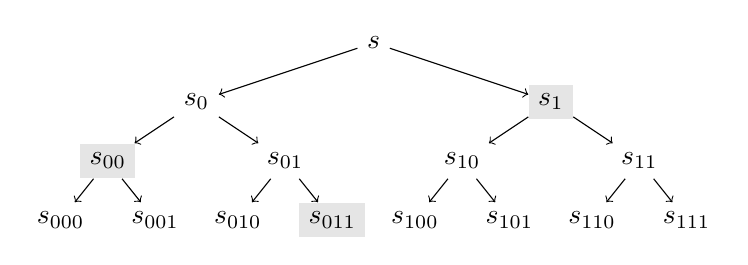
\begin{tikzpicture}[xscale=1.5, yscale=-.75]
	\tikzstyle{hl}=[fill=black!10!]
		\node (s) at (0,0) {$s$};
		
		\node (s0) at (-1.5, 1) {$s_0$};
		\node[hl] (s1) at (1.5, 1) {$s_1$};
		
		\node[hl] (s00) at (-2.25, 2) {$s_{00}$};
		\node (s01) at (-0.75, 2) {$s_{01}$};
		\node (s10) at (0.75, 2) {$s_{10}$};
		\node (s11) at (2.25, 2) {$s_{11}$};
		
		\node (s000) at (-2.25-.4, 3) {$s_{000}$};
		\node (s001) at (-2.25+.4, 3) {$s_{001}$};
		\node (s010) at (-0.75-.4, 3) {$s_{010}$};
		\node[hl] (s011) at (-0.75+.4, 3) {$s_{011}$};
		\node (s100) at (0.75-.4, 3) {$s_{100}$};
		\node (s101) at (0.75+.4, 3) {$s_{101}$};
		\node (s110) at (2.25-.4, 3) {$s_{110}$};
		\node (s111) at (2.25+.4, 3) {$s_{111}$};
		
		%========================================================================
		% Arrows
		\draw[->] (s) to (s0);
		\draw[->] (s) to (s1);
		
		\draw[->] (s0) to (s00);
		\draw[->] (s0) to (s01);
		\draw[->] (s1) to (s10);
		\draw[->] (s1) to (s11);
		
		\draw[->] (s00) to (s000);
		\draw[->] (s00) to (s001);
		\draw[->] (s01) to (s010);
		\draw[->] (s01) to (s011);
		\draw[->] (s10) to (s100);
		\draw[->] (s10) to (s101);
		\draw[->] (s11) to (s110);
		\draw[->] (s11) to (s111);
	\end{tikzpicture}
	\caption{\cite{CCS:KPTZ13} punctured PRF. Highlighted nodes constitute the key obtained puncturing in $x = (0,1,0)$.}
	\label{fig:KPTZ13:punctured_ggm}
\end{figure}

For ease of presentation we deviate from \cite{CCS:KPTZ13} and only show how to restrict the PRF on \textit{fixed prefix} strings, i.e. given $u \in \{0,1\}^\ell$ and a punctured key for $u$, we can only evaluate it on those $x = (u, v)$ for $v \in \{0,1\}$.
The final construction to puncture on a single point $x^\ast$ follows taking the union of keys for all prefixes $u$ of $x^\ast$ with the last bit of $u$ switched\footnote{In general given punctured keys $(k_1, \ldots, k_n)$ for $S_1, \ldots, S_n$ their union may not be a secure key punctured on $S_1 \cap \ldots \cap S_n$, but in this specific case it is.}.
A full description is provided in Figure~\ref{prot:KPTZ13:prefix_punctured_prf}.
For simplicity of notation, given a string $x = (b_1, \ldots, b_\ell)$ we will denote $G_x = G_{b_\ell} \circ \ldots \circ G_{b_1}$, with $G_0$ and $G_1$ being respectively the first and last $\secp$ bits of $G$'s output.

\begin{figure}[htb]
\centering
\begin{pcarray}{lll}
	\algorithm{
		$\cd{Gen}(1^\secp):$
		}
		{
			Sample a seed $s$
				\\
			\textbf{Return} $(s, \varnothing)$
		}
		&
	\algorithm{
		$\cd{Puncture}((s, \varnothing); u):$
		}
		{
			\textbf{Return} $G_u(s)$
		}
		&
	\algorithm{
		$\cd{Eval}((k, u), x)$
		}
		{
			Parse $x = (u', v)$
				\\
			\textbf{If} $u \neq u'$: \textbf{Return} $\perp$
				\\
			\textbf{Else}: \textbf{Return} $G_{v}(k)$
		}
\end{pcarray}
\caption{Punctured PRF from a PRG $G: \{0,1\}^\secp \to \{0,1\}^{2\secp}$. $G_0$ and $G_1$ on input $s$ returns respectively the first and last $\secp$ bits of $G(s)$. $\varnothing$ is used to denote the empty string.}
\label{prot:KPTZ13:prefix_punctured_prf}
\end{figure}

\begin{theorem}
	\label{theo:KPTZ13:prefix_punctured_prf}
	If $G : \{0,1\}^\secp \to \{0,1\}^{2\secp}$ is a secure PRG, then $(\cd{Gen}, \allowbreak \cd{Puncture}, \allowbreak \cd{Eval})$ is a puncturable PRF for the sets $\{S_u : u \in \cup_{\ell = 1}^n \{0,1\}^\ell\}$ where $S_u = \{x \: : \: \nexists v : x = (u, v)\}$.
\end{theorem}
\begin{proof}
	Correctness easily follows as given a key $s$ and its puncturing $k$ in $S_u$, then for all $x \notin S_u$, i.e. for all strings with prefix $u$, the evaluation with $k$ yields, calling $x = (u, v)$.
	\begin{align*}
		G_{v}(k)
			\; = \;
		G_v \circ G_u (s)
			\; = \;
		G_{(u,v)}(s)
			\; = \;
		G_x(s).
	\end{align*}
	To show pseudorandomness on punctured points, let $(k,u) = \cd{Puncture}(s, u)$ and $x \in S_u$. As $u$ is not a prefix of $x$, let $w$ be longest common prefix of $u$ and $x$.
	Without loss generality we assume the next bit after $w$ of $u$ to be $0$ while for $x$ to be $1$.
	Then we argue using the PRG security that the two distributions
	\[
		(G_{(w,0)}(s), G_{(w,1)}(s))
			, \quad
		(r_0, r_1)
	\]
	are computationally indistinguishable for random $r_0, r_1$. This follows as the first distribution is $G \circ G_w(s)$ that is a composition of PRGs.
	We thus conclude that the following distributions are computationally indistinguishable, where $u = (w, 0, \bar{u})$ and $x = (w, 1, \bar{u})$.
	\[
		\left( G_u(s),  G_x(s) \right)
			\; \equiv_c \;
		\left( G_{\bar{u}}(r_0), G_{\bar{x}}(r_1) \right)
			\; \equiv_c \;
		\left( G_{\bar{u}}(r_0), r^\ast \right)
	\]
	for uniformly sampled and independent $s, r_0, r_1, r^\ast$.
\end{proof}
	
\chapter{Hashing}
	\section{Chameleon Hash}
	%!TeX root = ../../ccc_main.tex
%!TeX spellcheck = en_GB

\subsection{From Claw-Free Permutation}

The first general construction of chameleon hash functions was provided in \cite{NDSS:KraRab00} based on claw-free trapdoor permutations \EG{ref}. 
First of all they observe that any chameleon hash with small message space can be extended over the set of all strings by composing with a collision-resistant hash function.
This clearly preserves collision resistance and, given a trapdoor for the underlying smaller chameleon hash, for any $y$ in the output space and $m \in \{0, 1\}^\ast$ one can find the right $r$ such that $(h(m), r)$ is mapped to $y$.

Next, they provide a chameleon hash applying to a random element $r$ subsequently either $f_0$ or $f_1$ according to the $i$-th bit of $m$, where $(f_0, f_1)$ is the pair of trapdoor permutations.
If an adversary manages to find a collision this directly translate into a claw for $f_0, f_1$.

\begin{figure}[htb]
\centering
\begin{pcarray}{l}
	\algorithm{
		$\cd{Setup}:$
		}
		{
			Sample permutations $f_0, f_1$ and trapdoors $f_0^{-1}, f_1^{-1}$
				\\
			$\cd{key} \gets (f_0, f_1), \; \cd{td} \gets (f_0^{-1}, f_1^{-1})$.
			Return $(\cd{key}, \cd{td})$
		}
		\\
	\algorithm{
		$\cd{Hash}(m, r, \cd{key}):$
		}
		{
			Parse $m = (b_1, \ldots, b_n)$ with $b_i \in \{0, 1\}$
				\\
			$y \gets f_{b_n} \circ \ldots \circ f_{b_1} (r)$. Return $y$
		}
		\\
	\algorithm{
		$\cd{Forge}(y, m, \cd{td}):$
		}
		{
			Parse $m = (b_1, \ldots, b_n)$ with $b_i \in \{0, 1\}$
				\\
			$r \gets f_{b_1}^{-1} \circ \ldots \circ f_{b_n}^{-1}(y)$. Return $r$
		}
\end{pcarray}
\caption{Chameleon hash from claw-free permutations in \cite{NDSS:KraRab00}, with $m \in \{0, 1\}^n$}
\label{prot:KraRab:trapdoor_permutations}
\end{figure}

\begin{proposition}
	If $f_0, f_1$ is a pair of claw-free trapdoor permutations, then the construction in figure \ref{prot:KraRab:trapdoor_permutations} is a chameleon hash
\end{proposition}


\subsection{From Factoring}
In \cite{NDSS:KraRab00} a concrete chameleon hash is provided based on the hardness of factoring by roughly instantiating the generic construction based on claw-free trapdoor permutations.
To do so they simply provide such a primitive whose claw-freeness is implied by factoring.
This is done by setting, for a given RSA modulus $N = pq$ with $p = 3 \mod 8$ and $p = 7 \mod 8$ by setting
\[	
	f_0 : \QR \to \QR
		\: : \:
	f_0(x) = x^2,
		\qquad
	f_1 : \QR \to \QR
		\: : \:
	f_1(x) = 4 x^2.
\]
The restriction imposed on $p, q$ guarantees that $-1$ is not a square both modulo $p$ and $q$, $2$ is not a quadratic residue $\mod p$ but it is $\mod q$.
Notice that knowing the factorisation of $N$ one can invert those functions by computing through chinese remainder theorem a square root that is itself a quadratic residue.
In conclusion one can prove the following

\begin{proposition}
	If factoring is hard then $f_0, f_1$ is a pair of claw-free trapdoor permutations on $\QR$
\end{proposition}

However deciding membership in $\QR$ is hard so an adversary breaking the resulting chameleon hash obtain directly from \ref{prot:KraRab:trapdoor_permutations} may find collision for values of $r \in \Z_N \setminus \QR$ leaving the reduction unable to tell whether this is a valid collision which translate into a claw for $f_0, f_1$.
For this reason one need to adapt the general construction by composing with $g : \Z_N \to \QR$ such that $g(x) = x^2$.

\begin{figure}[htb]
\centering
\begin{pcarray}{l}
	\algorithm{
		$\cd{Setup}:$
		}
		{
			$p, q \rgets \{0, 1\}^\ell$ primes s.t. $p \bmod 8 = 3, \; q \bmod 8 = 7$
				\\
			$N \gets pq, \; \cd{key} \gets N, \; \cd{td} \gets (p, q)$. Return $\cd{key}, \cd{td}$
		}
		\\
	\algorithm{
		$\cd{Hash}(m, r, \cd{key}):$
		}
		{
			Parse $m = (b_1, \ldots, b_n)$ with $b_i \in \{0, 1\}$
				\\
			$y \gets f_{b_n} \circ \ldots \circ f_{b_1} (r^2)$. Return $y$
		}
		\\
	\algorithm{
		$\cd{Forge}(y, m, \cd{td}):$
		}
		{
			Parse $m = (b_1, \ldots, b_n)$ with $b_i \in \{0, 1\}$
				\\
			$r \gets f_{b_1}^{-1} \circ \ldots \circ f_{b_n}^{-1}(y)$. Return $r$
		}
\end{pcarray}
\caption{Chameleon hash from factoring in \cite{NDSS:KraRab00}, $m \in \{0, 1\}^n$}
\label{prot:KraRab:factoring}
\end{figure}

\begin{proposition}
	If factoring is hard, the construction in Figure \ref{prot:KraRab:factoring} is a chameleon hash function
\end{proposition}

\subsection{From Discrete Log}
Still in \cite{NDSS:KraRab00} a chameleon hash based on discrete log is proposed. The idea could be generalised to produce chameleon hash from any perfectly hiding equivocal commitment.
This scheme however achieve mildly weaker forging property as $\cd{Forge}$ algorithm requires in input not only an image $y$ but also the message and randomness used to generate it.

\begin{figure}[htb]
\centering
\begin{pcarray}{l}
	\algorithm{
		$\cd{Setup}:$
		}
		{
			$g \rgets \G, \; x \rgets \F_q, \; h \gets g^x$
				\\
			$\cd{key} \gets (g, h), \; \cd{td} \gets x$. Return $\cd{key}, \cd{td}$
		}
		\\
	\algorithm{
		$\cd{Hash}(m, r, \cd{key}):$
		}
		{
			$y \gets g^m h^r$. Return $y$
		}
		\\
	\algorithm{
		$\cd{Forge}((y, m', r'), m, \cd{td}):$
		}
		{
			$r \gets r' + x^{-1}(m' - m)$. Return $r$
		}
\end{pcarray}
\caption{Chameleon hash from Discrete Log in \cite{NDSS:KraRab00}, $m \in \F_q$. Procedure $\cd{Forge}$ requires $m', r'$ such that $y = \cd{Hash}(m', r', \cd{key})$}
\label{prot:KraRab:dlog}
\end{figure}

\begin{proposition}
	If the discrete logarithm problem is hard in $\G$, the construction in Figure \ref{prot:KraRab:dlog} is a chameleon hash function
\end{proposition}










\chapter{Public Key Encryption}
	\section{Security against Chosen Plaintext Attack}
	\subsection{Stolbunov from Group Actions}

In the context of hard homogeneous space, a generalization of cryptographic groups which models a group action on a set (without assuming the set is also a group), the first encryption scheme was proposed by \cite{OTHER:Stolbunov10*}.
First let us recall the notation.
Given a group $\G$ and a set $\mathcal{E}$ the actions is denoted as
\[
	\star : \G \times \mathcal{E} \to \G
\]
with the assumption that $\mathcal{E}$ is a single orbit, that is $\mathcal{E} = \G \star E_0$ for some $E_0 \in \mathcal{E}$.
The following scheme assumes $\G$ to be commutative and the action faithful, that is each $E \in \mathcal{E}$ admit one and only one $a \in \G$ such that $a \star E_0 = E$.

The main obstacle to instantiate ElGamal encryption over HHS is that $(g^r, h^r \cdot m)$ with $m$ group element cannot be computed as we do not have a group operation.
The solution in \cite{OTHER:Stolbunov10*} is, using a DDH-like assumption, to compute the ciphertext from $r \star E_0, r \star E_x$, with $E_x = x \star E_0$ the public key and $x$ the secret key.
Next, to use the randomness in $r \star E_x$ an \textit{entropy smoothing} hash function $H_k : \mathcal{E} \to \{0, 1\}^\mu$ is used, whose security requirement is that, given a random key $k \in K$, input $x$ and image $y \in \{0, 1\}^\mu$, no $\ppt$ adversary can distinguish $(k, H_k(x))$ from $(k, y)$.
\EG{Add example of ES function}

%Notice that we do not require collision resistance. Hence an example of entropy-smoothing function family is, assuming $\mathcal{E} \subseteq \{0, 1\}^\nu$, the set of all linear maps in $\F_2^{\mu, \nu}$.

\begin{figure}[htb]
\centering
\begin{pcvstack}[center, space = 6pt]
\begin{pchstack}[center, space=12pt]
	\algorithm{
		$\cd{Setup}:$
		}
		{
			$k \rgets K$ key of the ES hash
				\\
			$x \rgets \G$
				\\
			$\pk = E_x \gets x \star E_0, \; \sk = x$
				\\
			Return $(\pk, \sk)$
		}
	\algorithm{
		$\cd{Enc}(m, \pk):$
		}
		{
			Sample $r \rgets \G$
				\\
			$c \gets (r \star E_0, H_k(r \star E_x) \oplus m)$
				\\
			Return $c$
		}
\end{pchstack}
\begin{pchstack}[center]
	\algorithm{
		$\cd{Dec}(c, \sk):$
		}
		{
			Parse $c = (E_r, \hat{c})$ with $E_r \in \mathcal{E}$ and $\hat{c} \in \{0, 1\}^\mu$
				\\
			Return $m \gets \hat{c} \oplus H_k(x \star E_r)$
		}
\end{pchstack}
\end{pcvstack}
\label{prot:Stolbunov10}
\caption{\cite{OTHER:Stolbunov10*} encryption for HHS, with message space $\{0, 1\}^\mu$}
\end{figure}

Correctness hold as we assumed $\G$ is commutative, since $r \star E_x = (r \cdot x) \star E_0 = (x \cdot r) \star E_0 = x \star E_r$. 
In particular their hash value is the same and so
\[
	\hat{c} \oplus H_k(x \star E_r)
		\; = \;
	m \oplus H_k(r \star E_x) \oplus H_k(x \star E_r)
		\; = \;
	m.
\]

Security holds under a DDH-like assumption over HHS \EG{check for a name, the proof goes through two hybrids, the first changes $r \star E_x$ with $E_z$ random and the second one replace $H_k(E_z)$ random with randomness. Then it becomes one time pad.}
	\subsection{Sahai-Waters from iO}

An important question on the path to render iO the "central hub" of modern cryptography is under which assumptions it implies fundamental primitives such as public-key encryption.
The first answer was provided by \cite{STOC:SahWat14}.
Their idea is to start with a simple secret key encryption from PRF $f$, which encrypts $m$ as $(r, f_k(r) \oplus m)$ with $r$ a random nonce.
Then this scheme is compiled into a public-key one.
The ingredients required for such transformation are
\begin{itemize}
	\item A puncturable PRF ($\cd{PRF.Gen}, \cd{PRF.Puncture}, \cd{PRF.Eval}$) \EG{cite}
	\item A pseudo-random generator $g : \{0,1\}^\secp \to \{0,1\}^{2\secp}$
	\item Indistinguishability obfuscation $\io$
\end{itemize}
Given the above $f_k(\cdot)$ is replaced with $\cd{PRF.Eval}(k, \cdot)$.
The randomness $r$ instead is sampled through $g(s)$ with short seed $s$, which creates a (relatively sparse) subset of "obtainable ciphertexts" in the space of all "valid" ones.
With these modifications, the public key of the resulting scheme is set as the obfuscation of the circuit evaluating the secret-key encryption.
\[
	C_k(m, s) = \left(
		g(s),
			\,
		\cd{PRF.Eval}(k, g(s)) \oplus m
	\right).
\]
The full scheme is described in figure \ref{prot:SahWat14:pke_from_io}.

\begin{figure}[htb]
	\centering
	\begin{pchstack}[center, space=12pt]
	\algorithm{
		$\cd{Gen}(1^\secp):$
		}
		{
			Sample $k \rgets \cd{PRF.Gen}(1^\secp)$
				\\
			Obfuscate $\tilde{C} \gets \io(C_k)$
				\\
			$\pk \gets \tilde{C}, \, \sk \gets k$
				\\
			\textbf{Return} $(\pk, \sk)$
		}
	\algorithm{
		$\cd{Enc}(\pk, m):$
		}
		{
			Sample a PRG seed $s$
				\\
			$c \gets \tilde{C}(m, s)$
				\\
			\textbf{Return} $c$
		}
	\end{pchstack}
	\begin{pchstack}[center, space=12pt]
	\algorithm{
		$\cd{Dec}(\sk, c):$
		}
		{
			Parse $c = (c_1, c_2)$
				\\
			\textbf{Return} $\cd{PRF.Eval}(k, c_1) \oplus c_2$
		}
	\end{pchstack}
	\label{prot:SahWat14:pke_from_io}
	\caption{Circuit evaluating the modified encryption scheme.}
\end{figure}

\begin{proposition}
	\label{prop:SahWat98}
	If $(\cd{PRF.Gen}, \cd{PRF.Puncture}, \cd{PRF.Eval})$ is a secure puncturable PRF, $g$ is a PRG and $\io$ is an indistinguishability obfuscator for P/poly, then the scheme in Figure~\ref{prot:SahWat14:pke_from_io} is IND-CPA secure.
\end{proposition}
\begin{proof}
	The proof follows from a sequence of four hybrid games, where we call $m_0, m_1$ the challenge messages chosen by the adversary and $b$ the bit sampled by the challenger.
	\begin{itemize}
		\item[$\cd{H}_0$:] The real IND-CPA game with $c = (g(s), \cd{PRF.Eval}(k, g(s)) \oplus m_b)$.
		
		\item[$\cd{H}_1$:] As $\cd{H}_0$ but $r^\ast$ is initially sampled and the challenge ciphertext is set as $c = (r^\ast, \cd{PRF.Eval}(k, r^\ast) \oplus m_b)$.
		
		\item[$\cd{H}_2$:] As $\cd{H}_1$ but $k^\ast \gets \cd{PRF.Puncture}(k, \{r^\ast\})$ and $\tilde{C} = \io(C_{k^\ast})$.
		
		\item[$\cd{H}_3$:] As $\cd{H}_2$ but $c = (r^\ast, z^\ast)$ with $z^\ast$ uniformly random.
	\end{itemize}
	At a high level $\cd{H}_0 \approx \cd{H}_1$ based on the PRG security replacing $g(s)$ with $r^\ast$.
	$\cd{H}_1 \approx \cd{H}_2$ uses the fact that, since $r^\ast$ is sampled uniformly over $\{0,1\}^{2\secp}$, the probability that $r^\ast \in \Im g$ is $2^{-\secp}$.
	Thus, conditioning on $r^\ast \notin \Im g$ we have that $C_k$ and $C_{k^\ast}$ are functionally equivalent.
	In particular the hybrid are indistinguishable due to the security of the obfuscator.
	Finally, from the pseudo-randomness of the PRF, as $k^\ast$ is punctured in $r^\ast$, the value $\cd{PRF.Eval}(k^\ast, r^\ast)$ is computationally indistinguishable from true randomness form the adversary's view.
	In particular so is $\cd{PRF.Eval}(k^\ast, r^\ast) \oplus m_b$.
\end{proof}





	\section{Security against Chosen Ciphertext Attack}
	%!TeX root = ../../ccc_main.tex
%!TeX spellcheck = en_GB

\subsection{Cramer-Shoup}

The first asymmetric encryption scheme proven $\cd{IND-CCA2}$ secure in the plain model under standard assumptions, namely $\ddh$ and the existence of target collision-resistant hash functions, was the Cramer-Shoup cryptosystem \cite{C:CraSho98}. Later reformulations generalized their construction to Hash Proof System \cite{EC:CraSho02} which can be based on a broader class of decisional problems.
The scheme is presented in Figure \ref{prot:CraSho98}. There $\gexp{}{x} = g^x$ with $g$ being the generator of a group $\G$ with prime order $q$ and $H : \{0,1\}^\ast \to \F_q^2$ denote a TCR \EG{ref} hash function such that any two distinct vector in its image are linearly independent.
This last requirement is not restrictive since, if $h : \{0, 1\} \to \F_q^2$ is a TCR, then $H(x) \coloneqq (1, h(x))$ is a TCR with the above property.
For simplicity in the scheme decryption we omit the hash function's key, implicitly sampled during the setup.

\begin{figure}[htb]
\centering
\begin{pcarray}{lll}
	\algorithm{
	$\cd{Setup}:$
	}
	{
		$\vc{w} \rgets \F_q^2, \quad \vc{x} \rgets \F_q^2, \quad A \rgets \F_q^{2,2}$
			\\
		$
			\pk \gets \left(
				\gexp{}{\vc{w}}
					, \,
				\gexp{}{\vc{w}^\trs \vc{x}}
					, \,
				\gexp{}{\vc{w}^\trs A}
				\right), \quad
			\sk \gets
				(\vc{x}, \, A)
		$
			\\
		Return $\pk, \sk$
	}
	\\
	\algorithm{
	$\cd{Enc}(M, \pk):$
	}
	{
		$s \rgets \F_q$
			\\
		\label{step:CraSho98:enc:first_part}
		$\vc{c}_0 \gets \gexp{}{s \vc{w}}
			, \quad
		c_1 \gets \gexp{}{s \vc{w}^\trs \vc{x}} \cdot M$
			\\
		\label{step:CraSho98:enc:second_part}
		$\vc{v} \gets H(\vc{c}_0, c_1), \quad c_2 \gets \gexp{}{s \vc{w}^\trs A \vc{v}}$
			\\
		Return $c \gets (\vc{c}_0, c_1, c_2)$
	}
	\\
	\algorithm{
	$\cd{Dec}(c, \sk, \pk):$
	}
	{
		Parse $c = (\vc{c}_0, c_1, c_2) \in \G^4$ and set $\vc{v} \gets H(\vc{c}_0, c_1)$
			\\
		\label{step:CraSho98:dec:test}
		\textbf{If} $c_2 \neq \vc{c}_0^{A \vc{v}}$: Return $\perp$
			\\
		\label{step:CraSho98:dec:decrypytion_step}
		Return $m \gets c_1 \cdot \vc{c}_0^{-\vc{x}}$	
	}
\end{pcarray}
\caption{$\cd{IND-CCA2}$ secure scheme in \cite{C:CraSho98}}
\label{prot:CraSho98}
\end{figure}

\begin{proposition}
	\label{prop:CraSho98}
	The scheme detailed in Figure \ref{prop:CraSho98} is $\cd{IND-CCA2}$ if $H$ is a TCR hash function and $\ddh$ holds in $\G$.
\end{proposition}

\begin{proof}[Proof of \ref{prop:CraSho98}]
	We propose the same hybrid games sequence of the original paper, but in a different order to make the argument more linear to follow.
	In the following $(\tilde{\vc{c}}_0, \tilde{c}_1, \tilde{c}_2)$ denotes the challenge ciphertext
	
	\paragraph{Hybrid Games}
	\begin{itemize}
	\item $\cd{G}_0$: The real game \EG{ref}.
	
	\item $\cd{G}_1$: The encryption oracle change $\cd{Enc}$ by setting $c_1 \gets \vc{c}_0^{\vc{x}} \cdot M$ and $c_2 \gets \vc{c}_0^{A \vc{v}}$.
	
	\item $\cd{G}_2$: The encryption oracle change $\cd{Enc}$ by sampling $\vc{c}_0 \rgets \G^2$.
	
	%\item $\cd{G}_3$: The decryption oracle change $\cd{Dec}$ by rejecting before line \ref{step:CraSho98:dec:test} if, after the challenger ciphertext has been requested, $(\vc{c}_0, c_1) \neq (\tilde{\vc{c}}_0, \tilde{c}_1)$ but $H(\vc{c}_0, c_1) = H(\tilde{\vc{c}}_0, \tilde{c}_1)$.
	
	\item $\cd{G}_3$: The decryption oracle change $\cd{Dec}$ by computing $\vc{w}^\perp$, $\vc{w}^\ast$ such that $\vc{w}^\trs \vc{w}^\perp = 0$, $\vc{w}^\trs \vc{w}^\ast = 1$ replacing the check on line \ref{step:CraSho98:dec:test} with
	\[
		\vc{c}_0^{\vc{w}^\perp} = 1
			\quad \wedge \quad
		(\vc{c}_0^{\vc{w}^\ast})^{\vc{w}^\trs A \vc{v}} = c_2
	\]
	and finally, replacing the step on line \ref{step:CraSho98:dec:decrypytion_step} with $m \rgets c_1 \cdot (\vc{c}_0^{\vc{w}^\ast})^{-\vc{w}^\trs \vc{x}}$.
	
	%\item $\cd{G}_5$: Change $\cd{Enc}$ by sampling $c_1 \rgets \G$.
	\end{itemize}
	
\begin{claim}
	\label{claim:CraSho98:G0-G1}
	$\cd{G}_0$ and $\cd{G}_1$ are identically distributed.
\end{claim}

\begin{claim}
	\label{claim:CraSho98:G1-G2}
	For any $\ppt$ algorithm $\mathcal{A}$ that distinguishes $\cd{G}_1$ from $\cd{G}_2$, there exists $\mathcal{B}$ $\ppt$ that breaks $\ddh$ over $\G$ with the same advantage $\varepsilon_1$ of $\mathcal{A}$.
\end{claim}

\begin{claim}
	\label{claim:CraSho98:G3 is hard}
	In game $\cd{G}_3$, up to negligible probability $1/q$, $\tilde{c}_1 \sim U(\G)$ and is independent from other group elements sent by the challenger and the adversary's random coins
\end{claim}	
	
\begin{claim}
	\label{claim:CraSho98:TCR}
	For any $\ppt$ algorithm $\mathcal{A}$ that in game $\cd{G}_3$ sends, after requesting the challenge ciphertext, a decryption query $(\vc{c}_0, c_1, c_2)$ such that $(\vc{c}_0, c_1) \neq (\tilde{\vc{c}}_0, \tilde{c}_1)$ but $H(\vc{c}_0, c_1) = H(\tilde{\vc{c}}_0, \tilde{c}_1)$ with probability $\varepsilon_2'$, there exists $\mathcal{C}$ that breaks the TCR of $H$ with probability $\varepsilon_2$ such that $\varepsilon_2' \leq \varepsilon_2 + q^{-1}$.
\end{claim}
	
\begin{claim}
	\label{claim:CraSho98:G2-G3}
	For any $\ppt$ algorithm $\mathcal{A}$ that distinguishes $\cd{G}_2$ from $\cd{G}_3$, calling $Q$ a polynomial bound on the number of decryption queries requested by $\mathcal{A}$, then its advantage is smaller than $Q \cdot q^{-1}$.
\end{claim}

Observe that by Claim \ref{claim:CraSho98:G3 is hard} in $\cd{G}_3$ all messages sent are independent from the challenge bit $b$, meaning that the advantage of any adversary is $0$. Applying the claims we deduce that the advantage of any $\ppt$ adversary to win the $\cd{IND-CCA2}$ is smaller than $\varepsilon_1 + \varepsilon_2 + (Q + 1) \cdot q^{-1}$.

\begin{claimproof}{\ref{claim:CraSho98:G0-G1}}
	The first two games $\cd{G}_0, \cd{G}_1$ are identically distributed since
	\begin{gather*}
	c_1	
		\; = \;
	\gexp{}{s \cdot \vc{w}^\trs \vc{x}} \cdot M
		\; = \;
	\gexp{}{s \cdot \vc{w}}^{\vc{x}} \cdot M
		\; = \;
	\vc{c}_0^{\vc{x}} \cdot M
		\\
	c_2
		\; = \;
	\gexp{}{s \cdot \vc{w}^\trs A \vc{v}}
		\; = \;
	\gexp{}{s \cdot \vc{w}}^{A \vc{v}}
		\; = \;
	\vc{c}_0^{A \vc{v}}.
	\end{gather*}
\end{claimproof}

\begin{claimproof}{\ref{claim:CraSho98:G1-G2}}
	Algorithm $\mathcal{B}$ breaking $\ddh$ is detailed in figure \ref{prot:CraSho98:DDH_reduction}
\begin{figure}[htb]
\centering
\algorithm{\textbf{Algorithm} $\mathcal{B}(\vc{g}, \vc{h})$}{
	Sample $\vc{x} \rgets \F_q^2$, $A \rgets \F_q^{2, 2}$ and set
	$\pk \gets \left( \vc{g}, \vc{g}^\vc{x}, \vc{g}^A \right), \; \sk \gets (\vc{x}, A)$
		\\
	Execute $\mathcal{A}(1^\secp, \pk)$
		\\
	When $\mathcal{A}$ request the decryption of $c$:
		\\
	\t Set $m \gets \cd{Dec}(c, \sk, \pk)$ and send $\mathcal{A} \gets m$
		\\
	When $\mathcal{A}$ request the encryption of $(M_0, M_1)$:
		\\
	\t Sample $b \rgets \{0, 1\}$; Set $\vc{c}_0 \gets \vc{h}, \; c_1 \gets \vc{c}_0^\vc{x} \cdot M_b$
		\\
	\t Set $\vc{v} \gets H(\vc{c}_0, c_1)$ and $c_2 \gets \vc{c}_0^{A \vc{v}}$; Send $\mathcal{A} \gets (\vc{c}_0, c_1, c_2)$
		\\
	When $\mathcal{A} \to b'$: Return $b'$.
}
\label{prot:CraSho98:DDH_reduction}
\caption{Algorithm $\mathcal{B}$ reducing the indistinguishability of $\cd{G}_1$-$\cd{G}_2$ to $\ddh$}
\end{figure}

	In both game $\ddh[0]$ and $\ddh[1]$ there exists a random $\vc{w} \in \F_q^2$ such that $\vc{g} = \gexp{}{\vc{w}}$, which implies that the public key is computed correctly. In $\ddh[1]$, there exists $s \sim U(\F_q)$ such that $\vc{h} = \vc{g}^s = \gexp{}{s \vc{w}}$ which means that the challenge ciphertext is as in $\cd{G}_1$
	\[
		\vc{c}_0 = \gexp{}{s \vc{w}}
			, \qquad
		c_1 = \vc{c}_0^\vc{x} \cdot M_b = \gexp{}{s \vc{w}^\trs \vc{x}} \cdot M_b
			, \qquad
		c_2 = \vc{c}_0^{A \vc{v}} = \gexp{}{s \vc{w}^\trs A \vc{v}}.
	\]
	In $\ddh[0]$ instead $\vc{h} = \vc{c}_0 \sim U(\G^2)$ which implies that the challenge ciphertext is distributed as in $\cd{G}_2$. In conclusion $\mathcal{A}$ and $\mathcal{B}$ share the same advantage.
\end{claimproof}

\begin{claimproof}{\ref{claim:CraSho98:G3 is hard}}
	Observe that beside the generation of the challenge ciphertext throughout the protocol the only information given about $\vc{x}$ is $\vc{w}^\trs \vc{x}$ that explicitly appears in the public key and is used in the decryption algorithm.\\
	Calling $\tilde{\vc{c}}_0 = \gexp{}{\vc{u}}$ with $\vc{u} \sim \G^2$, the probability that $\vc{u} = s \vc{w}$ for some $s \in \F_q$ is $q^{-1}$.
	Hence up to this negligible probability, $\vc{u}$ and $\vc{w}$ are linearly independent and, in particular $\vc{u}^\trs \vc{x}$ is statistically independent from $\vc{w}^\trs \vc{x}$. 
	It follows that $\tilde{c}_1 = \tilde{\vc{c}}_0^{\vc{x}} \cdot M_b = \gexp{}{\vc{u}^\trs \vc{x}} \cdot M_b$ is uniform over $\G$.
\end{claimproof}

\begin{claimproof}{\ref{claim:CraSho98:TCR}}
	Algorithm $\mathcal{C}$ breaking the TCR of $H$ is detailed in figure \ref{prot:CraSho98:TCR}
	
\begin{figure}[htb]
	\centering
	\algorithm{\textbf{Algorithm $\mathcal{C}$:}}{
		Sample $\vc{w} \rgets \F_q^2$, $\alpha \rgets \F_q$, $A \rgets \F_q^{2, 2}$ and $\vc{u} \rgets \F_q^2$ s.t. $\vc{w}$ and $\vc{u}$ are l.i.
			\\
		Compute $\vc{w}^\perp$ and $\vc{w}^\ast$ such that $\vc{w}^\trs \vc{w}^\perp = 0$ and $\vc{w}^\trs \vc{w}^\ast = 1$.
			\\
		Set $\tilde{\vc{c}}_0 \gets \gexp{}{\vc{u}}, \; \tilde{c}_1 \rgets \G$; send $(\tilde{\vc{c}_0}, \tilde{c}_1)$ to the challenger.
			\\
		Upon receiving $H$, set $\pk = \left( \gexp{}{\vc{w}}, \gexp{}{\alpha}, \gexp{}{\vc{w}^\trs A} \right)$; Send $\mathcal{A} \gets \pk$
			\\
		When $\mathcal{A}$ requests the encryption of $(M_0, M_1)$:
			\\
		\t $\vc{v} \gets H(\tilde{\vc{c}}_0, \tilde{c}_1), \; \tilde{c}_2 \gets \tilde{\vc{c}}_0^{A \vc{v}}$. Send $\mathcal{A} \gets (\tilde{\vc{c}}_0, \tilde{c}_1, \tilde{c}_2)$
			\\
		When $\mathcal{A}$ requests the decryption of $(\vc{c}_0, c_1, c_2)$:
			\\
		\t If $(\vc{c}_0, c_1) \neq (\tilde{\vc{c}}_0, \tilde{c}_1)$ and $H(\vc{c}_0, c_1) = H(\tilde{\vc{c}}_0, \tilde{c}_1)$: Return $(\vc{c}_0, c_1)$
			\\
		\t If $\vc{c}_0^{\vc{w}^\perp} \neq 1$ or $(\vc{c}_0^{\vc{w}^\ast})^{\vc{w}^\trs A \vc{v}}$ with $\vc{v} \gets H(\vc{c}_0, c_1)$: Send $\mathcal{A} \gets \perp$
			\\
		\t Otherwise $m \gets c_1 \cdot (\vc{c}_0^{\vc{w}^\ast})^{-\alpha}$. Send $\mathcal{A} \gets m$.
	}
	\label{prot:CraSho98:TCR}
	\caption{Algorithm $\mathcal{C}$ breaking the TCR of $H$}
\end{figure}
	
	Calling $\tilde{c}_1 = \gexp{}{\beta}$ it follows by the linearly independence of $\vc{u}$ and $\vc{w}$ that there exists a unique $\vc{x} \in \F_q^2$ such that $\alpha = \vc{w}^\trs \vc{x}$ and $\beta = \vc{u}^\trs \vc{x}$.
	Hence $\mathcal{C}$ correctly simulates $\cd{G}_3$ conditioned to $\vc{u}$ and $\vc{w}$ being linearly independent -- which does not occur with probability $q^{-1}$.
	The claim is therefore proven since the if and only $\mathcal{C}$'s output is a target collision for $H$, the event in the statement occurs if and only if $\mathcal{C}$ finds a collision for $H$
\end{claimproof}

\begin{claimproof}{\ref{claim:CraSho98:G2-G3}}
	First of all we observe that the actual decryption is identical in the two experiments, when it does not return an error, because
	\begin{multline*}
		\vc{c}_0^{\vc{w}^\perp} \neq 1
			\quad \ra \quad
		\exists s : \vc{c}_0 = \gexp{}{s \vc{w}}
			\quad \ra \quad
		c_1 \cdot (\vc{c}_0^{\vc{w}^\ast})^{-\vc{w}^\trs \vc{x}}
			\; = \\
			= \;
		c_1 \cdot \gexp{}{s (\vc{w}^\trs \vc{w}^\ast) \cdot (-\vc{w}^\trs \vc{x})}
			\; = \;
		c_1 \cdot \gexp{}{s \vc{w}}^{-\vc{x}}
			\; = \;
		c_1 \cdot \vc{c}_0^{- \vc{x}}.
	\end{multline*}
	Hence the only way to distinguish the two worlds is to submit a decryption query accepted in $\cd{G}_2$ but rejected in $\cd{G}_3$. We show that for each query this can happen at most with probability $q^{-1}$.\\
	In general, when $(\vc{c}_0, c_1, c_2)$ is accepted in $\cd{G}_2$ but rejected in $\cd{G}_3$ then we cannot have $\vc{c}_0^{\vc{w}^\trs} = 1$ or, otherwise $\exists s : \vc{c}_0 = \gexp{}{s \vc{w}}$ and
	\[
		(\vc{c}_0^{\vc{w}^\ast})^{\vc{w}^\trs A \vc{v}}
			\; = \;
		\gexp{}{s (\vc{w}^\trs \vc{w}^\ast) \cdot (\vc{w}^\trs A \vc{v})}
			\; = \;
		\gexp{}{s \vc{w}}^{A \vc{v}}
			\; = \;
		\vc{c}_0^{A \vc{v}}
			\; = \;
		c_2.
	\]
	Hence $\vc{c}_0^{\vc{w}^\trs} \neq 1$. Call $\vc{r} \in \F_q^2$ its exponent, i.e. $\vc{c}_0 = \gexp{}{\vc{r}}$, and $t$ the exponent of $c_2$. By our assumption that the query is accepted in $\cd{G}_2$ we have that $t = \vc{r}^\trs A \vc{v}$.\\
	We are now ready to study two cases:\\
	
	\textit{Case 1: The query occurs before the challenge ciphertext is requested}. In this case the only information known to an unbounded adversary $\mathcal{A}$ about $A$ is $\vc{w}^\trs A$, present in the public key and used in the decryption algorithm. As $\vc{r}$ and $\vc{w}$ are linearly independent and $A \sim U(\F_q^{2, 2})$ the vectors $\vc{w}^\trs A$ and $\vc{r}^\trs A$ are uniform over $\G^2$ and independent.\\
	To prove it formally, the matrix $M = (\vc{w}, \vc{r})$ is invertible, implying that for any $B \in \F_q^2$ there is a unique solution $A \in \F_q^2$ such that $M^\trs A = B$.\\
	Hence $t \sim U(\G)$ and the adversary can correctly guess it only with probability $q^{-1}$.\\
	
	\textit{Case 2: the query occurs after the challenge ciphertext is requested}. Call
	\[
		\tilde{\vc{c}}_0 = \gexp{}{\vc{u}}
			, \quad
		\tilde{c}_1 = \gexp{}{\vc{u}^\trs \vc{x}} \cdot M_b
			, \quad
		\tilde{c}_2 = \gexp{}{\vc{u}^\trs A \tilde{\vc{v}}}
	\]
	the challenge ciphertext components. By the way $\cd{IND-CCA2}$ is defined, $(\vc{c}_0, c_1, c_2) \neq (\tilde{\vc{c}}_0, \tilde{c}_1, \tilde{c}_2)$. If by contradiction the first two entries of these tuples were equal, then, from the assumption that the first one is accepted in $\cd{G}_2$
	\[
		H(\vc{c}_0, c_1)
			\; = \;
		H(\tilde{\vc{c}}_0, \tilde{c}_1)
			\quad \ra \quad
		c_2
			\; = \;
		\vc{c}_0^{A \vc{v}}
			\; = \;
		\tilde{\vc{c}_0}^{A \tilde{\vc{v}}}
			\; = \;
		\tilde{c}_2.
	\]
	Therefore $(\vc{c}_0, c_1) \neq (\tilde{\vc{c}}_0, \tilde{c}_1)$ and by Claim \ref{claim:CraSho98:TCR}, up to negligible probability, their hash $\vc{v}$, $\tilde{\vc{v}}$ are distinct. Moreover, by our assumptions on $H$, $\vc{v}$ and $\tilde{\vc{v}}$ are linearly independent.\\
	When $\vc{w}$ and $\vc{u}$ are l.i.\footnote{if they are not the adversary only knows $\vc{w}^\trs A$ and we fall back to case 1} the adversary's information on $A$ consist of $\vc{w}^\trs A$ and $\vc{w}^\trs A \tilde{\vc{v}}$, which is equivalent to $\vc{w}^\trs A$ and $\vc{r}^\trs A \tilde{\vc{v}}$ as $\{\vc{w}, \vc{u}\}$ and $\{\vc{w}, \vc{r}\}$ are both bases.
	This implies that $\vc{r}^\trs A \vc{v}$ is uniform and independent even conditioning on the above values as, calling $M = (\vc{w}, \vc{r})$ and $V = (\tilde{\vc{v}}, \vc{v})$, the system $M^\trs A V = B$ as a unique solution for any $B \in \F_q^{2, 2}$. It follows that $t \sim U(\F_q)$ and the adversary can only correctly guess it with probability $q^{-1}$.
	
	\end{claimproof}
	

\end{proof}
	
	\section{Lossy Encryption}
	\subsection{PVW Lossy Encryption from DDH}
\EG{NOTE: we use the group in additive notation}
Although the formal definition of \textit{lossy encryption} was first given in \cite{AC:HLOV11}, the first construction and motivations dates back to \cite{C:PeiVaiWat08}.
In that paper the primitive was presented as \textit{dual-mode} encryption where the public key can be generated in two indistinguishable ways.
In \textit{injective} mode, each ciphertext produced with it preserves the plaintext and allows for correct decryption.
Conversely in \textit{messy} or \textit{lossy} mode, encryption retain almost no information on the message.

In the following we present a slightly modified version of their scheme based on DDH.
First, it generalizes ElGamal to the group $\G^2$ for regular encryption, with public key in injective mode being $\vc{g}, \vc{h}$ with $\vc{h} = x \cdot \vc{g}$. Concretely, for message $m \in \G$ and randomness $\vc{r} \in \F_q^2$
\[
	\vc{c} = \left( \vc{r}^\trs \vc{g}, \; \vc{r}^\trs \vc{h} + m \right)
\]
Conversely lossy keys are generated choosing $\vc{g}, \vc{h}$ both random.
The idea is that in this way the encryption of any message will be uniformly distributed over the ciphertext space even if the discrete logarithms of $\vc{g}$ and $\vc{h}$ are known.
The full construction presented in Figure~\ref{prot:PVW08}

\begin{figure}[htb]
\centering
\begin{pcarray}{ll}
	\algorithm{
		$\cd{Setup}(1^\secp):$
		}
		{
			$\sk = x \rgets \F_q$ the secret key
				\\
			$\vc{g} \rgets \G^2, \; \vc{h} \gets x \cdot \vc{g}$
				\\
			Return $(\pk, \sk)$ with $\pk = (\vc{g}, \vc{h})$	
		}
	&
	\algorithm{
		$\cd{LossySetup}(1^\secp):$
		}
		{
			$\vc{g}, \vc{h} \rgets \G^2$
				\\
			Return $\pk = (\vc{g}, \vc{h})$
		}
	\\
	\algorithm{
		$\cd{Enc}(m, \pk)$
		}
		{
			Parse $\pk = (\vc{g}, \vc{h})$
				\\
			Sample $\vc{r} \rgets \F_q^2$
				\\
			$c_1 \gets \vc{r}^\trs \vc{g}, \; c_2 \gets \vc{r}^\trs \vc{h} + m$
				\\
			Return $\vc{c} = (c_1, c_2)$
		}
	&
	\algorithm{
		$\cd{Dec}(c, \sk):$
		}
		{
			Parse $c = (c_1, c_2) \in \G^2$
				\\
			Return $m \gets c_1 - x \cdot c_2$
		}
\end{pcarray}
\label{prot:PVW08}
\caption{\cite{C:PeiVaiWat08} encryption for HHS, with message space ${0, 1}^\mu$}
\end{figure}

\begin{proposition}
	\label{prop:GVW08}
	The scheme described in Figure~\ref{prot:PVW08} is an IND-CPA secure lossy encryption scheme if DDH is hard.
\end{proposition}
\begin{proof}
	\EG{TODO: IND-CPA is like el-gamal. Key indistinguishability is plain DDH. Lossiness comes for the fact that for any $m$ the map $\vc{r} \mapsto \cd{Enc}(\pk, m; \vc{r})$ is surjective}
\end{proof}


\chapter{Signatures}
	\section{Digital Signatures Schemes}
	%!TeX root = ../../ccc_main.tex
%!TeX spellcheck = en_GB

\subsection{Hohenberger-Waters RSA Short Signature}
The first efficient RSA signature produced without relying on tree structures was presented in \cite{C:HohWat09}. Their construction make use of the generic transformation from weakly-secure signatures and a chameleon hash function \EG{refs, especially for the RSA chameleon hash}.
In order to produce a weak signature they introduce the \textit{prefix-guessing} technique, which allows in the security reduction to sign required messages while still being able to retrieve non-trivial information from a forge.

At a high level for any message $m \in \{0, 1\}^n$ let $m^{(i)}$ be its prefix of length $i$, i.e. its first $i$ bits. 
If the adversary requires signatures of $m_1, \ldots, m_Q$ and forges a messages $\hat{m}$, then there exists at least a message $m_{i^\ast}$ with the longest common prefix with $\hat{m}$.
In other words $\hat{m}^{(t^\ast)} = m_{i^\ast}^{(t^\ast)}$.
The reduction can then correctly guess $i^\ast$ and $t^\ast$ with significant probability and ``embed'' the challenge in all those message whose $t^\ast$ first bits agree with $m_{i^\ast}$ and the $t^\ast + 1$-th don't, while still being able to simulate the other messages.
Notice that the $m_i$ don't satisfy this requirement, and that knowing them in advance (even before producing public parameters) is essential to correctly produce this partition.

Finally they apply this technique using a programmable target collision-resistant hash function $H : \{0, 1\}^\ast \to \{0, 1\}^\ell$ mapping strings to prime numbers.
This can be obtained from a PRF. 
A key a PRF's key $k$ and $c \rgets \{0, 1\}^\ell$ and $H(m) \coloneqq f_k(j, m) \oplus c$ where $j$ is the smallest integer that makes $f_k(j, m) \oplus c$ a prime number.

\begin{figure}[htb]
\centering
\begin{pcvstack}
	\algorithm{
		$\cd{Setup}:$
		}
		{
			Sample $H$ programmable TCR hash function
				\\
			$p_1, p_2 \rgets \range{2^\ell}$ primes, $\;$ $N \gets p_1 \cdot p_2$, $\;$ $h \rgets \Z_N^\ast$
				\\
			$\vk \gets (H, N, h), \; \sk \gets \phi(N)$. Return $\vk, \sk$
		}
	\algorithm{
		$\cd{Sign}(m, \sk):$
		}
		{
			Set $m^{(i)}$ the first $i$ bits of $m \in \{0, 1\}^n$
				\\
			$e_i \gets H(m^{(i)}), \quad \sigma \gets h^{e_1^{-1} \cdot \ldots \cdot e_n^{-1}}$
				\\
			Return $\sigma$
		}
	\algorithm{
		$\cd{Vfy}(m, \sigma, \cd{vk}):$
		}
		{
			Set $m^{(i)}$ the first $i$ bits of $m \in \{0, 1\}^n$
				\\
			$e_i \gets H(m^{(i)}. \;$ Return $h \checkeq \sigma^{e_1 \cdot \ldots \cdot e_n}$
		}
\end{pcvstack}
\label{prot:HohWat09}
\caption{Short RSA signature \cite{C:HohWat09}. $H$ maps to primes of length $\ell$}
\end{figure}

\begin{proposition}
	\label{prop:HohWat09}
	The scheme detailed in Figure \ref{prot:HohWat09} is a weakly secure signature if the RSA problem is hard.
\end{proposition}

	\subsection{Sahai-Water Short Signature from iO}
An fundamental question in the study of digital signatures regards the efficiency gap between their secret-key counterpart.
In particular MAC can be as short as a single PRF output.
The first construction showing that Digital signature can achieve the same length, at the price of slower verification time, was presented in \cite{STOC:SahWat14}.
Their construction however achieves only \textit{selective security}, namely, the adversary must declare the message $m^\ast$ he intends to produce a forgery of before the public parameters are generated.

The construction is based on a puncturable PRF $(\cd{PRF.Gen}, \allowbreak \cd{PRF.Eval}, \allowbreak \cd{PRF.Puncture})$ (we denote $F_k = \cd{PRF.Eval}$), a one-way function $f$ and indistinguishability obfuscation $\io$.
The idea is to lift the PRF-as-MAC \EG{cite?} construction obfuscating the verification procedure.
Puncturing the PRF on the message chosen by the adversary ideally allows to argue that no information on a signature at that point is given to the adversary.
However \textit{some} information must be embedded in the circuit, or else there would be no valid signature for $m^\ast$ after puncturing, which renders the punctured program functionally different from the correct one.

To solve the issue "degraded" (but sufficient for authentication) information on $F_k(m^\ast)$ is embedded, which allow for verification but does not allow to fully retrieve $F_k(m^\ast)$.
This is simply $f(F_k(m^\ast))$.
The verification circuit is then defined as
\[
	C_k(m, \sigma)
		\; \coloneqq \;
	f(\sigma) == f(F_k(m)).
\]
The scheme is described in Figure~\ref{prot:SahWat14:short_signature_from_io}.

\begin{figure}[htb]
	\centering
	\begin{pchstack}[center, space=10pt]
	\algorithm{
		$\cd{Gen}(1^\secp):$
		}
		{
			$k \rgets \cd{PRF.Gen}(1^\secp)$
				\\
			$\tilde{C} \rgets \io(C_k)$
				\\
			\textbf{Return} $(\vk, \sk) = (\tilde{C}, k)$
		}
	\algorithm{
		$\cd{Sign}(\sk, m):$
		}
		{
			\textbf{Return} $F_k(m)$
		}
	\algorithm{
		$\cd{Vfy}(\vk, \sigma):$
		}
		{
			Parse $\vk = \tilde{C}$
				\\
			\textbf{Return} $\tilde{C}(m, \sigma)$	
		}
	\end{pchstack}
	\label{prot:SahWat14:short_signature_from_io}
	\caption{Short Signatures from iO presented in \cite{STOC:SahWat14}.}
\end{figure}

\begin{theorem}
	\label{theo:SahWat14:short_signatures_from_io}
	If $(\cd{PRF.Gen}, \cd{PRF.Eval}, \cd{PRF.Puncture})$ is a puncturable PRF, $f$ a one-way function, and $\io$ a secure obfuscator for P/poly, then the signature scheme in Figure~\ref{prot:SahWat14:short_signature_from_io} is selectively unforgeable.
\end{theorem}
\begin{proof}
	The proof goes through three hybrids. First let $C^\ast_{k^\ast, m^\ast, z^\ast}$ be the circuit returning
	\[
	C^\ast_{k^\ast, m^\ast, z^\ast}(m, \sigma)
		\; = \;
	\begin{cases}
		f(\sigma) == z^\ast & \text{If } m^\ast = m
			\\
		f(\sigma) == f(F_{k^\ast}(m)) & \text{If } m^\ast \neq m
	\end{cases}.
	\]
	Given the above we define the three hybrids:
	\begin{itemize}
	\item{$\cd{H}_0$:} The real unforgeability game.
	
	\item{$\cd{H}_1$:} As $\cd{H}_0$, but $k^\ast$ is computed as $\cd{PRF.Puncture}(k, \{m^\ast\})$, $z^\ast = f(F_k(m^\ast))$ and $\tilde{C}$ is the obfuscation of $C^\ast_{k^\ast, m^\ast, z^\ast}$.
	
	\item{$\cd{H}_2$:} As $\cd{H}_1$, but $z^\ast$ is computed as $f(r^\ast)$ with $r^\ast$ a random value.
	\end{itemize}
	
	Intuitively, the first two hybrids are indistinguishable as $C_k$ and $C^\ast_{k^\ast, m^\ast, z^\ast}$ are functionally equivalent.
	$\cd{H}_1 \approx \cd{H}_2$ follows as $F_k(m^\ast)$ is indistinguishable from random given the adversary's view, which is now a function of the \textit{punctured} key.
	Finally, unforgeability in $\cd{H}_2$ follows from the hardness of the OWF.
	Indeed any forgery $\sigma$ for $m^\ast$, is a valid preimage for $f(r^\ast)$.
\end{proof}
	
	\section{Verifiable Random Functions (VRF)}	
	\EG{Just a road map}
Papers list
\begin{itemize}
	
	\item \cite{PKC:DodYam05}: Compact VRF with "small" message space (or "long" proofs) from q-SDH. (Not sure why the message space has to be small in their construction).

	\item \cite{EPRINT:EKSSZSC20}: Efficient from lattices, introduces the Game-based notion of unbiasability.
	
	\item \cite{EPRINT:EEKLSSYZ22}: Indexed VRF (for forward security). Extends the notion of unbiasability to this setting.	
\end{itemize}
	\subsection{From Verifiable Unpredictable Functions}

The original paper \cite{FOCS:MicRabVad99} introducing the notion of VRF, further presented a general construction from Verifiable Unpredictable Functions \EG{cite}.
The result is broken into three steps: first a $1$-bit selectively secure\footnote{Such that the challenge input is queried before generating the public parameters.} VRF is built using the Goldreich-Levin hardcore predicate \cite{STOC:GolLev89}.
Next, through complexity leveraging we can obtain a VRF with super-polynomial (but possibly not exponential) input and output space.
Finally, large input space is achieved through a tree-like construction.

Let the starting VUF have output space in $\{0,1\}^n$.
The idea is to generate $(\vk, \sk)$ the VUF parameters along with a random string $r \in \{0,1\}^n$ and set the VRF output to be $y^\trs r$ with $y$ the VUF output.
The construction is presented in Figure~\ref{prot:MRV99:sel_sec_vrf_from_vuf}

\begin{figure}[htb]
	\centering
	\begin{pcvstack}[center, space=10pt]
	\begin{pchstack}[center, space=10pt]
	\algorithm{
		$\cd{VRF.Gen}(1^\secp)$
		}
		{
			$\vk, \sk \rgets \cd{VUF.Gen}(1^\secp)$
				\\
			$r \rgets \{0,1\}^n$
				\\
			$\vk^\ast \gets (\vk, r), \; \sk^\ast \gets \sk$
				\\
			\textbf{Return} $((\vk, r), \sk)$
		}
	\algorithm{
		$\cd{VRF.Eval}(\sk, x)$
		}
		{
			$y \gets \cd{VUF.Eval}(\sk, x)$
				\\
			$y^\ast \gets y^\trs r$
				\\
			$\pi^\ast \gets y$
				\\
			\textbf{Return} $(y^\ast, \pi^\ast)$	
		}
	\end{pchstack}
	\begin{pchstack}
	\algorithm{
		$\cd{VRF.Vfy}(\vk^\ast, x, y^\ast, \pi^\ast)$
		}
		{
			Parse $\vk^\ast = (\vk, r)$
				\\
			\textbf{Return} $1$ if:
				\\
			\t $y^\ast = (\pi^\ast)^\trs r$
				\\
			\t $1 = \cd{VUF.Vfy}(\vk, x, \pi^\ast)$
		}
	\end{pchstack}
	\end{pcvstack}
	\label{prot:MRV99:sel_sec_vrf_from_vuf}
	\caption{VUF to selectively secure VRF compiler in \cite{FOCS:MicRabVad99}.}
\end{figure}

\begin{theorem}
	\label{theo:MRV99:vuf_to_sel_secure_vrf}
	Let $(\cd{VUF.Gen}, \cd{VUF.Eval}, \cd{VUF.Vfy})$ be a VUF. Then the construction in Figure~\ref{prot:MRV99:sel_sec_vrf_from_vuf} is a selectively secure VRF with the same input space and output space $\{0,1\}$.
\end{theorem}
\begin{proof}
	\EG{TODO}
\end{proof}
	
	
\chapter{Functional Encryption}
	\section{Identity Based Encryption}
	%!TeX root = ../../ccc_main.tex
%!TeX spellcheck = en_GB

\subsection{Boneh-Franklin IBE}

In \cite{C:BonFra01} the first two construction of an IBE scheme in the random oracle model were presented. 
\EG{revise - is this customary?}
In the following let $e : \G_1 \times \G_2 \to \G_T$ be a pairing of prime order $q$ groups, $g_1, g_2, g_T$ their generators and $\ro : \{0,1\}^\ast \to \G_2$ the random oracle.

\begin{figure}[htb]
\centering
\begin{pcarray}{lll}
	\algorithm{
		$\cd{Setup}:$
		}
		{
			$s \rgets \F_q, \quad h \rgets g_1^s$
				\\
			$\mpk \gets h, \quad \msk \gets s$
				\\
			Return $\mpk, \msk$
		}
	&
	\algorithm{
		$\cd{KeyGen}(\cd{id}, \msk):$
		}
		{
			$Q_\cd{id} \gets \ro(\cd{id}), \quad \sk_\cd{id} \gets Q_\cd{id}^s$
				\\
			Return $\sk_\cd{id}$
		}
	\\
	\algorithm{
			$\cd{Enc}(m, \cd{id}, \mpk):$
			}
			{
				$r \rgets \F_q, \quad Q_\cd{id} \gets \ro(\cd{id})$
					\\
				$c_0 \gets g_1^r, \quad c_1 \gets m \cdot e(h^r, Q_\cd{id})$
					\\
				Return $(c_0, c_1)$
			}
	&
	\algorithm{
		$\cd{Dec}(c, \sk_\cd{id}, \mpk):$
		}
		{
			Parse $c = (c_0, c_1)$
				\\
			$m \gets c_1 \cdot e(c_0, \sk_\cd{id})^{-1}$
				\\
			Return $m$
		}
\end{pcarray}
\caption{First IBE scheme proposed in \cite{C:BonFra01}}
\label{prot:BonFra01:first}
\end{figure}

This scheme is correct as $e(c_0, \sk_\cd{id}) = e(g_1^r, Q_\cd{id})^s = e(h^r, Q_\cd{id})$. Indistinguishability under chosen plaintext attack instead can be proven under the $\cd{BDH}$ assumption \EG{ref}.
\begin{proposition}
	\label{prop:BonFra01:first}
	The scheme \ref{prot:BonFra01:first} is an $\cd{IND-CPA}$ Identity Based Encryption scheme under the $\cd{BDH}$ assumption in the Random Oracle Model.
\end{proposition}
Using the Fujisaki-Okamoto transform \cite{C:FujOka99} the above construction can be turned into an $\cd{IND-CCA}$ secure scheme. Even though originally this black box transformation was designed for simple asymmetric encryption schemes, it can be applied in this context as well. Given two independent random oracles $\ro[0] : \{0, 1\}^\ast \to \F_q$ and $\ro[1] : \{0, 1\}^\ast \to \{0, 1\}^\ell$ the encryption of an $\ell$ bits message is performed by returning
\[
	\cd{Enc}(\sigma, \cd{id}, \mpk; \ro[0](\sigma, m))
		, \quad
	\ro[1](\sigma) \oplus m
\]
where $\sigma \sim U(\G_T)$ and $\cd{Enc}(\sigma, \cd{id}, \mpk; r)$ denotes the encryption of $\sigma$ with randomness $r$.
Decryption is carried out by extracting $\sigma$ from the first component using $\sk_\cd{id}$ and then $m$ by adding $\ro[1](\sigma)$ to the second component.
Finally, if the first term does not equal the encryption of $\sigma$ using randomness $\ro[0](\sigma, m)$, that is a deterministic procedure, the decryption algorithm fails returning $\perp$. Otherwise it returns the message $m$.
This modifications are all summarised in figure \ref{prot:BonFra01:second}.

\begin{figure}[htb]
\centering
\begin{pcarray}{ll}
	\procedure[mode = text, linenumbering]
	{$\cd{Enc}^\ast(m, \cd{id}, \mpk)$}{
		$\sigma \rgets \G_T, \quad c_1 \gets \ro[1](\sigma) \oplus m$
			\\
		$c_0 \gets \cd{Enc}(\sigma, \cd{id}, \mpk; \ro[0](\sigma, m))$
			\\
		Return $(c_0, c_1)$
	}
		&
	\procedure[mode = text, linenumbering]
	{$\cd{Dec}^\ast(c, \sk_\cd{id}, \mpk)$}{
		Parse $c = c_0, c_1$
			\\
		$\sigma \gets \cd{Dec}(c_0, \sk_\cd{id}, \mpk)$
			\\
		$m \gets c_1 \oplus \ro[1](\sigma)$
			\\
		\textbf{If} $c_0 \neq \cd{Enc}(\sigma, \cd{id}, \mpk; \ro[0](\sigma, m))$:
			\\
		\t Return $\perp$
			\\
		\textbf{Else}: Return $m$
	}
\end{pcarray}
\caption{Enhanced encryption and decryption procedure in \cite{C:BonFra01}}
\label{prot:BonFra01:second}
\end{figure}

\begin{proposition}
	The scheme $(\cd{Setup}, \cd{KeyGen}, \cd{Enc}^\ast, \cd{Dec}^\ast)$ detailed in Figures \ref{prot:BonFra01:first} and \ref{prot:BonFra01:second} is an $\cd{IND-CCA}$ IBE under the $\cd{BDH}$ assumption in the Random Oracle Model.
\end{proposition}

	%!TeX root = ../../ccc_main.tex
%!TeX spellcheck = en_GB

\subsection{Waters IBE}

The first construction in the standard model using constant assumptions is presented in \cite{EC:Waters05}. 
For simplicity, we present here the original version using symmetric pairings - even though it could be adapted to asymmetric ones.
Historically, this is one of the first constructions that successfully used a partitioning technique in order to simulate the secret key required, but at the same time embed the underlying problem in the challenge ciphertext.

\begin{figure}[htb]
\centering
\begin{pcarray}{lll}
	\algorithm{
		$\cd{Setup}:$
		}
		{
			$\alpha, \beta \rgets \F_q, \quad \vc{w} \rgets \F_q^{n+1}$
				\\
			$\mpk \gets (\gexp{}{\alpha}, \gexp{}{\beta}, \gexp{}{\vc{w}}),
				\quad
			\msk \gets \gexp{}{\alpha \beta}$
				\\
			Return $(\mpk, \msk)$
		}
	&
	\algorithm{
		$\cd{KeyGen}(\vc{d}, \msk):$
		}
		{
			$r \rgets \F_q$
				\\
			$\sk_\vc{d} \gets (\gexp{}{r}, \gexp{}{\alpha \beta + r \vc{w}^\trs \vc{d}})$
				\\
			Return $\sk_\vc{d}$
		}
	\\
	\algorithm{
			$\cd{Enc}(m, \vc{d}, \mpk):$
			}
			{
				$\rho \rgets \F_q$
					\\
				$c_0 \gets \gexp{}{\rho}
					, \quad 
				c_1 \gets \gexp{1}{\rho \vc{w}^\trs \vc{d}}$
					\\
				$c_2 \gets m \cdot e(\gexp{}{\alpha}, \gexp{}{\beta})^\rho$
					\\
				Return $(c_0, c_1, c_2)$
			}
	&
	\algorithm{
		$\cd{Dec}(c, \sk_\vc{d}, \mpk):$
		}
		{
			Parse $c = (c_0, c_1, c_2)$
				\\
			Parse $\sk_\vc{d} = (\sigma_1, \sigma_2)$
				\\
			$m \gets c_2 \cdot e(c_0, \sigma_2) \cdot e(c_1, \sigma_1)^{-1}$
				\\
			Return $m$
		}
\end{pcarray}
\caption{Waters IBE. Identities are of the form $\vc{d} \in \{1\} \times \{0, 1\}^n$}
\label{prot:Waters05:IBE}
\end{figure}

\begin{proposition}
	The scheme in Fig.~\ref{prot:Waters05:IBE} is an $\cd{IND-CPA}$ IBE under the $\cd{BDH}$ assumption
\end{proposition}

\begin{proof}[Proof sketch]
	In order to reduce security to the $\cd{BDH}$ problem, given an instance $h_1 = \gexp{}{\alpha}, h_2 = \gexp{}{\beta}, k = \gexp{}{\gamma}, c^\ast$, we need to build a simulator achieving two orthogonal goals:
	First he has to give secret keys for queried identities and second, he has to embed the problem in the challenge ciphertext.
	
	For the first goal, if we just set $\mpk = (h_1, h_2, \gexp{}{\vc{w}})$ succeeding in producing any key would imply breaking hard problems like $\cd{CDH}$. Our next best option is to sacrifice knowledge on the exponents $\vc{w}$ and $r$, for instance by setting
	\[
		\vc{w} = \vc{v} + \alpha \vc{x},
			\quad
		r = s + \beta y
	\]
	Then, the exponent of $\sk_\vc{d}$ becomes
	\begin{align*}
		\alpha \beta + (s + \beta y) \cdot(\vc{v} + \alpha \vc{x})^\trs \vc{d} 
			& \; =
		\alpha \beta 
			+ 
		s \cdot \vc{w}^\trs \vc{d} 
			+ 
		\beta y \cdot \vc{v}^\trs \vc{d} 
			+ 
		\alpha \beta y \cdot \vc{x}^\trs \vc{d}
	\end{align*}
	In order to cancel out $\alpha \beta$ we need $1 - y \vc{x}^\trs \vc{d} = 0$, which can be obtained by setting $y = -(\vc{x}^\trs \vc{d})^{-1}$ if this inner product is non-zero.
	For clarity, calling $\vc{u} = \gexp{}{\vc{v} + \alpha \vc{x}}$, one would compute the secret key by setting
	\[
		y \gets -\frac{1}{\vc{x}^\trs \vc{d}}
			, \qquad
		\sigma_0 \gets \gexp{}{r} \cdot h_2^{y}
			, \qquad
		\sigma_1 \gets 
			\vc{u}^{s \vc{d}}
				\cdot
			h_1^{y \cdot \vc{v}^\trs \vc{d}},
	\]
	and finally $\sk_\vc{d} \gets (\sigma_0, \sigma_1)$. 
	Next, to simulate the challenge ciphertext we can easily set $c_0 \gets k$ and $c_2 \gets m \cdot c^\ast$.
	The hard part is computing the middle term $c_2$. 
	It's exponent is $\rho \cdot \vc{v}^\trs \vc{d} + \rho \alpha \cdot \vc{x}^\trs \vc{d}$.
	Clearly we can compute the first term but not the second one. Hence, to make this step simulatable we need $\vc{x}^\trs \vc{d} = 0$.
	
	To sum up, calling $\vc{d}_1, \ldots, \vc{d}_Q$ the identity keys queried by the adversary and $\vc{d}_0$ the one used in the challenge, our simulation strategy works if
	\[
	\begin{cases}
		\vc{x}^\trs \vc{d}_i \neq 0 \quad \forall i \in \range{Q}
			\\
		\vc{x}^\trs \vc{d}_0 = 0
	\end{cases}
	.
	\]
	The proof's core is then showing how to chose $\vc{x}$ in such a way that the above condition happens with significant probability.
	This can be done either as shown in the original paper or with standard techniques from programmable hash functions \cite{C:HofKil08}.
\end{proof}
	
	\section{Inner Product Functionality}
	% Simple Inner Product FE
	%!TeX root = ../../ccc_main.tex
%!TeX spellcheck = en_GB

\subsection{ABDP Selectively Secure IPFE from DDH}
\EG{I'm using the group additively, this should be done in other examples too since the notation is much much clearer}
One of the first functional encryption scheme was proposed in \cite{PKC:ABDP15}.
The construction, which can be generalized to work with black box encryption schemes with certain homomorphic properties, can be summarized as a vector ElGamal encryption with common randomness.
The construction only uses a prime order group, with no pairings and of known order.
Notice that similarly to other group-based FE scheme, the decryption result is obtained in the exponent, and can then be retrieved by brute-force discrete logarithm algorithms efficiently as long as it lies in a polynomially bounded range.
In terms of security it is only selectively secure in the standard model, however it can be proved adaptively secure in the GGM \EG{not in the original paper, should I prove it?}.

\begin{figure}[htb]
\centering
\begin{pcarray}{lll}
	\algorithm{
		$\cd{Setup}(1^\secp, n):$
		}
		{
			$\vc{v} \rgets \F_q^n$
				\\
			$\mpk \gets \gexp{}{\vc{v}}, \quad \msk \gets \vc{v}$
				\\
			Return $(\mpk, \msk)$
 		}
	&
	\algorithm{
		$\cd{KeyGen}(\vc{d}, \msk):$
		}
		{
			Return $\sk_\vc{d} \gets \vc{d}^\trs \vc{v}$
		}
	\\
	\algorithm{
		$\cd{Enc}(\vc{x}, \mpk):$
		}
		{
			$s \rgets \F_q$
				\\
			$c \gets \left( \gexp{}{s}, 
				\; 
			\gexp{}{\vc{x} + s \vc{v}} \right)$
				\\
			Return $c$
		}
	&
	\algorithm{
		$\cd{Dec}(c, \sk_\vc{d}, \mpk):$
		}
		{
			Parse $c = (c_0, \vc{c}_1)$
				\\
			$m \gets \vc{d}^\trs \vc{c}_1 - \sk_\vc{d} \cdot c_0$
				\\
			Return $m$
		}
\end{pcarray}
\caption{ABDP Selectively Secure Inner Product Functional Encryption.}
\label{prot:ABDP15:IPFE}
\end{figure}

The scheme is correct since, using the same notation of Fig.~\ref{prot:ABDP15:IPFE}
\[
	m
		\; = \;
	\gexp{}{\vc{d}^\trs \vc{x} + s \cdot \vc{d}^\trs \vc{x}}
		-
	\gexp{}{s \cdot \vc{d}^\trs \vc{x}}
		\; = \;
	\gexp{}{\vc{d}^\trs \vc{x}}.
\]

\begin{proposition}
	The scheme in Fig.~\ref{prot:ABDP15:IPFE} is a Selectively Secure Functional Encryption with Inner Product functionality under the $\ddh$ assumption. 
\end{proposition}
\begin{proof}[sketch]
	We provide a direct reduction $\mathcal{B}$ to $\ddh$ given an adversary $\mathcal{A}$ for the indistinguishability game.
	On input $\gexp{}{\alpha}, \gexp{}{\beta}, \gexp{}{\gamma}$, $\mathcal{B}$ executes the adversary which will query $\vc{x}_0, \vc{x}_1$. Then it samples a random bit $b$ and compute the master public key and challenge ciphertext as
	\[
		\mpk
			\; = \;
		\gexp{}{\vc{u} + \alpha(\vc{x}_1 - \vc{x}_0)}
			\qquad
		c
			\; = \;
		\left( \gexp{}{\beta}, \; \gexp{}{\vc{x}_b + \beta \vc{u} + \gamma(\vc{x}_1 - \vc{x}_0)} \right)
	\]
	with $\vc{u}$ uniformly sampled over the linear space $V \subseteq \F_q^n$ orthogonal to $\vc{x}_1 - \vc{x}_0$.
	When the adversary queries the secret key for a vector $\vc{d}$ the reduction replies with
	\[
		\sk_\vc{d}
			\; = \;
		\vc{d}^\trs \vc{u}.
	\]
	Finally when the adversary guesses a bit $b'$ the reduction returns $1$ if the guess was correct, i.e. if $b' = b$, $0$ otherwise.
	
	Regardless of which experiment $\mathcal{B}$ is executed in, secret keys are generated correctly if $\mathcal{A}$ only performs legitimate queries, that are vectors $\vc{d}$ such that $\vc{d}^\trs \vc{x}_0 = \vc{d}^\trs \vc{x}_1$ as this implies $\vc{d}^\trs(\vc{x}_1 - \vc{x}_0)$ and in particular
	\[
		\sk_\vc{d}	
			\; = \;
		\vc{d}^\trs \vc{v}
			\; = \;
		\vc{d}^\trs \left( \vc{u} + \alpha(\vc{x}_1 - \vc{x}_0) \right)
			\; = \;
		\vc{d}^\trs \vc{u}.
	\]
	If $\mathcal{B}$ is executed in $\ddh[1]$, that is with $\gamma = \alpha \beta$, the challenge ciphertext is also correctly generated as the exponent of the second component becomes $\beta$ times the exponent of the master public key.
	Conversely if $\mathcal{B}$ is executed in $\ddh[0]$, $\gamma$ is uniformly random and in particular $\vc{x}_b + \gamma(\vc{x}_0 - \vc{x}_1)$ is uniformly distributed over the affine line containing $\vc{x}_0$ and $\vc{x}_1$.
	Thus $\mathcal{A}$ has no information on $b$ and cannot guess better than at random.
	In conclusion
	\begin{align*}
		\adv{\mathcal{B}}
			\; &= \;
		\left| \prob{\mathcal{A} \text{ wins} \,|\, \ddh[1]} - \prob{\mathcal{A} \text{ wins} \,|\, \ddh[0]} \right|
			\\ &= \;
		\left| \frac{1}{2} + \frac{1}{2} \cdot \adv{\mathcal{A}} - \frac{1}{2} \right|
			\; = \;
		\frac{1}{2} \cdot \adv{\mathcal{A}}.
	\end{align*}
\end{proof}
	%!TeX root = ../../ccc_main.tex
%!TeX spellcheck = en_GB

\subsection{Agrawal-Libert-Stehl\'{e} Adaptively Secure IPFE from DDH}

The main limitation of \cite{PKC:ABDP15} is that in the standard model only selective security can be achieved, an issue inherited by primitives based on it.
To address this issue, \cite{C:AgrLibSte16} proposed a variant achieving adaptive security at the cost of $1$ extra group element in ciphertexts and public key, and one extra field element in secret keys.
The system is inspired by the Cramer-Shoup cryptosystem \cite{C:CraSho98} or more generally Hash Proof Systems \cite{EC:CraSho02}.
At a high level the main observations they build upon are
\begin{enumerate}
	\item A \textit{private key} version of \cite{PKC:ABDP15}, where the challenger only encrypts the challenge ciphertext would be adaptively secure.
	In the security proof this is implicitly proven to be true information-theoretically.
	
	\item Using Hash Proof Systems it is possible to setup both a public key and private key instance of \cite{PKC:ABDP15} and at any time produce a ciphertext with the private-key system.
\end{enumerate}

A detailed description is given in Fig.~\ref{prot:AgrLibSth16:IPFE}.
Correctness follows since
\[
	m
		\; = \;
 	\gexp{}{\vc{d}^\trs \left(\vc{x} + A \vc{w} \right)}
 		-
 	\gexp{}{\vc{d}^\trs A \vc{w}}
 		\; = \;
 	\gexp{}{\vc{d}^\trs\vc{x}}.
\]

\begin{figure}[htb]
\centering
\begin{pcarray}{lll}
	\algorithm{
		$\cd{Setup}(1^\secp, n):$
		}
		{
			$A \rgets \F_q^{n, 2}, \; \vc{w} \rgets \F_q^2$
				\\
			$\mpk \gets \left( \gexp{}{\vc{w}}, \gexp{}{A\vc{w}} \right), \, \msk \gets \left(A, \vc{w}\right)$
				\\
			Return $(\mpk, \msk)$
		}
	&
	\algorithm{
		$\cd{KeyGen}(\vc{d}, \msk):$
		}
		{
			$\sk_\vc{d} \gets \vc{d}^\trs A$
				\\
			Return $\sk_\vc{d}$
		}
	\\
	\algorithm{
		$\cd{Enc}(\vc{x}, \mpk):$
		}
		{
			Sample $r \rgets \F_q$
				\\
			$c \gets \left(\gexp{}{r \vc{w}}, \gexp{}{\vc{x} + r A \vc{w}} \right)$
				\\
			Return $c$
		}
	&
	\algorithm{
		$\cd{Dec}(c, \sk_\vc{d}, \mpk):$
		}
		{
			Parse $c = (\vc{c}_0, \vc{c}_1) \in \G^2 \times \G^n$
				\\
			$m \gets \vc{d}^\trs \vc{c}_1 - \sk_\vc{d}^\trs \cdot \vc{c}_0$
				\\
			Return $m$
		}
\end{pcarray}
\caption{Agrawal-Libert-Sthel\'{e} Adaptively Secure IPFE from DDH.}
\label{prot:AgrLibSth16:IPFE}
\end{figure}

\begin{proposition}
	The scheme in Fig.~\ref{prot:AgrLibSth16:IPFE} is an Adaptively Secure Functional Encryption for Inner Production is $\ddh$ is hard in $\G$.
\end{proposition}
\begin{proof}
	First, we define the following hybrid games, with $b \sim U(\{0, 1\})$ being the bit used in the indistinguishability game \EG{ref}.
	\begin{itemize}
		\item $\cd{G}_0$: The real game \EG{ref?}.
		
		\item $\cd{G}_1$: As $\cd{G}_0$ but when the adversary submit the challenge messages $\vc{x}_0, \vc{x}_1$, the ciphertext is computed sampling $\vc{z} \rgets \F_q^2$ and setting
		\[
			c 
				\; = \; 
			\left( \gexp{}{\vc{z}}, \; \gexp{}{\vc{x}_b + A \vc{z}} \right).
		\]
	\end{itemize}
	We will first prove that $\cd{G}_0$ is indistinguishable from $\cd{G}_1$ using $\ddh$ and then that any adversary in $\cd{G}_1$ has negligible advantage $q^{-1}$.\\
	
	For the first part, let $\mathcal{A}$ be a distinguisher between $\cd{G}_0$ and $\cd{G}_1$. 
	We define $\mathcal{B}$ which breaks $\ddh$ using $\mathcal{A}$.
	On input $\gexp{}{\alpha}, \gexp{}{\beta}, \gexp{}{\gamma}$ it samples a random $\rho \rgets \F_q$, $A \rgets \F_q^{n, 2}$ and set
	\[
		\gexp{}{\vc{w}}
			\; = \;
		\gexp{}{(\rho, \alpha)}
			, \qquad
		\gexp{}{\vc{z}}
			\; = \;
		\gexp{}{(\rho\beta, \gamma)}.
	\]
	Thus it sets the master public key as $\gexp{}{\vc{z}}, \, \gexp{}{A \vc{z}}$ applying $A$ in the exponent.
	Key generation queries for $\vc{d}$ are answered with $\vc{d}^\trs A$ as prescribed while the challenge ciphertext is computed setting
	\[
		c 
			\; = \;
		\left( \gexp{}{\vc{w}}, \; \gexp{}{\vc{x}_b + A \vc{w}} \right)
	\]
	again applying $A$ in the exponent to get $\gexp{}{A \vc{w}}$.
	In $\ddh[1]$, $\mathcal{B}$ correctly simulates game $\cd{G}_0$ as $\gamma = \alpha \beta$ implies that $\vc{z} = \beta \vc{w}$ and in particular the challenge ciphertext is correctly distributed.
	Conversely in $\ddh[0]$, $\vc{w} \sim U(\F_q^2)$ and independently with other messages sent in the challenge, as in $\cd{G}_1$.
	Hence $\adv{\mathcal{B}} = \adv{\mathcal{A}}$.\\
	
	For the second part, up to a negligible probability $q^{-1}$, $\vc{z}$ and $\vc{w}$ are linearly independent.
	Conditioning on this event we show that the view of a given adversary $\mathcal{A}$ follows the same distribution when $b = 0$ or $b = 1$.
	Calling $\vc{y}_1, \ldots, \vc{y}_t$ all the key generation queries requested throughout the execution, and let $Y = (\vc{y}_1, \ldots, \vc{y}_t)$.
	Notice that $\vc{y}_i^\trs \vc{x}_0 = \vc{y}_i^\trs \vc{x}_1$ implies that $\vc{y}_i$ is orthogonal to $\vc{x}_1 - \vc{x}_0$ and in particular $Y^\trs(\vc{x}_1 - \vc{x}_0) = \vc{0}$.
	With this notation adversary's view is a function of 
	\[
		D_b \; = \; (A\vc{w}, \; Y^\trs A, \; \vc{x}_b + A \vc{z}).
	\]
	Since $\vc{w}, \vc{z}$ are linearly independent, there exists a matrix $B \in \F_q^{n, 2}$ such that $B \vc{w} = \vc{0}$ and $B \vc{z} = \vc{x}_1 - \vc{x}_0$.
	Given this matrix we conclude that $D_0$ and $D_1$ follows the same distribution since $A + B \sim U(\F_q^{n, 2})$ and, applying the transformation $A \mapsto A + B$ to $D_0$
	\[
		(A + B) \vc{w} 
			\, = \, 
		A \vc{w},
			\qquad
		Y^\trs(A + B)
			\, = \,
		Y^\trs A,
			\qquad
		\vc{x}_0 + (A + B) \vc{z}
			\, = \,
		\vc{x}_1 + A \vc{z}
	\]
	where the second equation follows as $Y^\trs B \in \F_q^{t, 2}$ is the zero matrix because it maps $\vc{z}, \vc{w}$ (a base of $\F_q^2$) to the zero vector.
	Thus $\adv{A} \leq q^{-1}$ in $\cd{G}_1$, concluding the proof.
\end{proof}
	% Function-Hiding Inner Product FE
	%!TeX root = ../../ccc_main.tex
%!TeX spellcheck = en_GB

%===============================================================================
% Local Commands
\newcommand{\IPsetup}{\cd{IP.Setup}}
\newcommand{\IPenc}{\cd{IP.Enc}}
\newcommand{\IPkeygen}{\cd{IP.KeyGen}}
\newcommand{\IPdec}{\cd{IP.Dec}}


%===============================================================================

\subsection{Lin's Weak Function Hiding Secret Key IPFE}
In \cite{C:Lin17}, Section 6, the first pairing-based rate-1 construction\footnote{i.e. such that to encrypt a vector of length $n$ the ciphertext has length $n + o(n)$.} of a function hiding IPFE was proposed.
This improved the previous construction \cite{AC:BisJaiKow15} which expanded encrypted vectors by a factor $2$ and returned upon decryption elements of the form
\[
	\gexp{T}{\theta}
		, \;
	\gexp{T}{\theta \cdot \vc{x}^\trs \vc{y}}
\]
with $\vc{x}$ being the encrypted vector and $\vc{y}$ the vector linked to the secret key.
Although this allows to recover $\vc{x}^\trs \vc{y}$ when this values is known to lie in a polynomially small set, it fails to cover the more general case of computing the generalized pairing
\[
	e(\gexp{1}{\vc{x}}, \gexp{2}{\vc{y}})
		\; = \;
	\gexp{T}{\vc{x}^\trs \vc{y}}.
\]
%
To solve this issue, \cite{C:Lin17} abandoned the dual pairing vector spaces paradigms of Okamoto and Takashima \cite{PAIRING:OkaTak08, AC:OkaTak09}, building instead almost generically upon the IPFE in \cite{PKC:ABDP15}.
The key properties of this scheme are:
\begin{enumerate}
	\item Decryption in \cite{PKC:ABDP15} consist of evaluating an ``inner product'' with ciphertext in $\G^{n+1}$ and secret key in $\F_q^{n+1}$.
	
	\item The decryption algorithm is linear in the vector $\vc{d}$ which describes the function.
	Thus, it can be generalized to vectors of group elements in $\G_1^n$ or $\G_2^n$.
\end{enumerate}
Given them, the core idea to encrypt $\vc{x}$ and generate a secret key for $\vc{y}$ is to apply the IPFE twice: 
$\vc{x}_0$ is first encrypted into $\gexp{1}{\vc{x}_1} \in \G_1^{n+1}$ while from $\vc{y}_0$ a related secret key $\vc{y}_1 \in \F_q^{n+1}$ is computed.
Next, having setted up a new instance of the IPFE for vectors of length $n+1$, in order to hide $\vc{y}_0$, $\vc{y}_1$ is encrypted into $\gexp{2}{\vc{y}_2} \in \G_2^{n+2}$ and $\gexp{1}{\vc{x}_1}$ is used as input in the key generation procedure to get $\gexp{2}{\vc{x}_2} \in \G_1^{n+2}$.
In this way performing a pairing inner product between $\vc{c}$ and $\sk_\vc{y}$ returns
\[
	\gexp{T}{\vc{x}_2^\trs \vc{y}_2}
		\; = \;
	\gexp{T}{\vc{x}_1^\trs \vc{y}_1}
		\; = \;
	\gexp{T}{\vc{x}^\trs \vc{y}}
\]
where all the equality follow as the result of each of these inner products is also the result of the respective decryption procedure.
More formally the scheme is described in Fig.~\ref{prot:Lin17:wfh_IPFE} explicitly.

\begin{figure}[htb]
\centering
\begin{pcarray}{lll}
	\algorithm{
		$\cd{Setup}(1^\secp, n):$
		}
		{
			$\vc{v}_1 \rgets \F_q^n, \; \vc{v}_2 \rgets \F_q^{n+1}$
				\\
			Return $\msk = (\vc{v}, \vc{w})$
 		}
	&
	\algorithm{
		$\cd{KeyGen}(\vc{y}, \msk):$
		}
		{
			Sample $r \rgets \F_q$
				\\
			$\vc{y}_1 \gets (-\vc{y}^\trs \vc{v}_1, \; \vc{y})$
				\\
			$\gexp{2}{\vc{y}_2} \gets \left(\gexp{2}{r}, \; \gexp{2}{\vc{y}_1 + r \vc{v}_2}\right)$
				\\
			Return $\sk = \gexp{2}{\vc{y}_2}$
		}
	\\
	\algorithm{
		$\cd{Enc}(\vc{x}, \msk):$
		}
		{
			Sample $s \rgets \F_q$
				\\
			$\gexp{1}{\vc{x}_1} \gets \left( \gexp{1}{s},\; \gexp{1}{\vc{x} + s \vc{v}_1} \right)$
				\\
			$\gexp{1}{\vc{x}_2} \gets \left( \gexp{1}{-\vc{x}_1^\trs \vc{v}_2},\; \gexp{2}{\vc{x}_1} \right)$
				\\
			Return $\vc{c} = \gexp{1}{\vc{x}_2}$
		}
	&
	\algorithm{
		$\cd{Dec}(\vc{c}, \sk):$
		}
		{
			Return $e(\vc{c}, \sk)$
		}
\end{pcarray}
\caption{Weakly secure function hiding IPFE in \cite{C:Lin17}.}
\label{prot:Lin17:wfh_IPFE}
\end{figure}

\begin{proposition}
	The scheme in Fig.~\ref{prot:Lin17:wfh_IPFE} is a weakly selectively secure function-hiding secret-key IPFE under the SXDH assumption. 
\end{proposition}
\begin{proof}[Proof sketch]
	\EG{TODO: Clarify the definition of selective security in this context (all queries are done together). This weak security notion comes from the usage of ABDP, which is only selectively secure.}
\end{proof}
	% Slotted Inner Product FE

%===============================================================================
% PART ?: Distributed systems and protocols
\part{Distributed Systems and Protocols}
\chapter{Consensus Protocols}
	%!TeX root = ../../ccc_main.tex
%!TeX spellcheck = en_GB

\begin{itemize}
	\setlength\itemsep{6pt}
	
	\item \cite{CCS:Reiter94}: Reliable broadcast. Dealer sends messages, parties echo with a signature and the dealer uses said signatures to convince others the broadcast succeeded.
\end{itemize}


%% Bibliography
\bibliographystyle{alpha}
\bibliography{cryptobib/abbrev3,cryptobib/crypto,others}

%% Appendix
\appendix

\end{document}
